%%%%%%%%%%%%%%%%%%%%%%%%%%%%%%%%%%%%%%%%%
% Thesis 
% LaTeX Template
% Version 1.3 (21/12/12)
%
% This template has been downloaded from:
% http://www.latextemplates.com
%
% Original authors:
% Steven Gunn 
% http://users.ecs.soton.ac.uk/srg/softwaretools/document/templates/
% and
% Sunil Patel
% http://www.sunilpatel.co.uk/thesis-template/
%
% License:
% CC BY-NC-SA 3.0 (http://creativecommons.org/licenses/by-nc-sa/3.0/)
%
% Note:
% Make sure to edit document variables in the Thesis.cls file
%
%%%%%%%%%%%%%%%%%%%%%%%%%%%%%%%%%%%%%%%%%

%----------------------------------------------------------------------------------------
%	PACKAGES AND OTHER DOCUMENT CONFIGURATIONS
%----------------------------------------------------------------------------------------

\documentclass[11pt, a4paper, oneside]{Thesis} % Paper size, default font size and one-sided paper

\graphicspath{{./Pictures/}} % Specifies the directory where pictures are stored
\usepackage{mathtools}
\usepackage[square, numbers, comma, sort&compress]{natbib} % Use the natbib reference package - read up on this to edit the reference style; if you want text (e.g. Smith et al., 2012) for the in-text references (instead of numbers), remove 'numbers' 
\hypersetup{urlcolor=blue, colorlinks=true} % Colors hyperlinks in blue - change to black if annoying
\title{\ttitle} % Defines the thesis title - don't touch this

\begin{document}
  

\frontmatter % Use roman page numbering style (i, ii, iii, iv...) for the pre-content pages

\setstretch{1.3} % Line spacing of 1.3

% Define the page headers using the FancyHdr package and set up for one-sided printing
\fancyhead{} % Clears all page headers and footers
\rhead{\thepage} % Sets the right side header to show the page number
\lhead{} % Clears the left side page header

\pagestyle{fancy} % Finally, use the "fancy" page style to implement the FancyHdr headers

\newcommand{\HRule}{\rule{\linewidth}{0.5mm}} % New command to make the lines in the title page

% PDF meta-data
\hypersetup{pdftitle={\ttitle}}
\hypersetup{pdfsubject=\subjectname}
\hypersetup{pdfauthor=\authornames}
\hypersetup{pdfkeywords=\keywordnames}


%----------------------------------------------------------------------------------------
% MACROS
%----------------------------------------------------------------------------------------

\DeclarePairedDelimiter{\ceil}{\lceil}{\rceil}
\newcommand{\footlink}[2]{\href{#1}{#2}\footnote{#1}}



%----------------------------------------------------------------------------------------
%	TITLE PAGE
%----------------------------------------------------------------------------------------

\begin{titlepage}
\begin{center}

\textsc{\LARGE \univname}\\[1.5cm] % University name
\textsc{\Large Master Thesis}\\[0.5cm] % Thesis type

\HRule \\[0.4cm] % Horizontal line
{\huge \bfseries \ttitle}\\[0.4cm] % Thesis title
\HRule \\[1.5cm] % Horizontal line
 
\begin{minipage}{0.4\textwidth}
\begin{flushleft} \large
\emph{Author:}\\
\href{http://www.johnsmith.com}{\authornames} % Author name - remove the \href bracket to remove the link
\end{flushleft}
\end{minipage}
\begin{minipage}{0.4\textwidth}
\begin{flushright} \large
\emph{Supervisor:} \\
\href{http://www.jamessmith.com}{\supname} % Supervisor name - remove the \href bracket to remove the link  
\end{flushright}
\end{minipage}\\[3cm]
 
\large \textit{A thesis submitted in fulfilment of the requirements\\ for the degree of \degreename}\\[0.3cm] % University requirement text
\textit{in the}\\[0.4cm]
\groupname\\\deptname\\[2cm] % Research group name and department name
 
{\large \today}\\[4cm] % Date
%
\includegraphics{Logo} % University/department logo - uncomment to place it
 
\vfill
\end{center}

\end{titlepage}

%----------------------------------------------------------------------------------------
%	DECLARATION PAGE
%	Your institution may give you a different text to place here
%----------------------------------------------------------------------------------------
% 
% \Declaration{
% 
% \addtocontents{toc}{\vspace{1em}} % Add a gap in the Contents, for aesthetics
% 
% I, \authornames, declare that this thesis titled, '\ttitle' and the work presented in it are my own. I confirm that:
% 
% \begin{itemize} 
% \item[\tiny{$\blacksquare$}] This work was done wholly or mainly while in candidature for a research degree at this University.
% \item[\tiny{$\blacksquare$}] Where any part of this thesis has previously been submitted for a degree or any other qualification at this University or any other institution, this has been clearly stated.
% \item[\tiny{$\blacksquare$}] Where I have consulted the published work of others, this is always clearly attributed.
% \item[\tiny{$\blacksquare$}] Where I have quoted from the work of others, the source is always given. With the exception of such quotations, this thesis is entirely my own work.
% \item[\tiny{$\blacksquare$}] I have acknowledged all main sources of help.
% \item[\tiny{$\blacksquare$}] Where the thesis is based on work done by myself jointly with others, I have made clear exactly what was done by others and what I have contributed myself.\\
% \end{itemize}
%  
% Signed:\\
% \rule[1em]{25em}{0.5pt} % This prints a line for the signature
%  
% Date:\\
% \rule[1em]{25em}{0.5pt} % This prints a line to write the date
% }
% 
% \clearpage % Start a new page

%----------------------------------------------------------------------------------------
%	QUOTATION PAGE
%----------------------------------------------------------------------------------------
% 
% \pagestyle{empty} % No headers or footers for the following pages
% 
% \null\vfill % Add some space to move the quote down the page a bit
% 
% \textit{``Thanks to my solid academic training, today I can write hundreds of words on virtually any topic without possessing a shred of information, which is how I got a good job in journalism."}
% 
% \begin{flushright}
% Dave Barry
% \end{flushright}
% 
% \vfill\vfill\vfill\vfill\vfill\vfill\null % Add some space at the bottom to position the quote just right
% 
% \clearpage % Start a new page

%----------------------------------------------------------------------------------------
%	ABSTRACT PAGE
%----------------------------------------------------------------------------------------

% \addtotoc{Abstract} % Add the "Abstract" page entry to the Contents
% 
% \abstract{\addtocontents{toc}{\vspace{1em}} % Add a gap in the Contents, for aesthetics
% 
% The Thesis Abstract is written here (and usually kept to just this page). The page is kept centered vertically so can expand into the blank space above the title too\ldots
% }
% 
% \clearpage % Start a new page

%----------------------------------------------------------------------------------------
%	ACKNOWLEDGEMENTS
%----------------------------------------------------------------------------------------
% 
% \setstretch{1.3} % Reset the line-spacing to 1.3 for body text (if it has changed)
% 
% \acknowledgements{\addtocontents{toc}{\vspace{1em}} % Add a gap in the Contents, for aesthetics
% 
% The acknowledgements and the people to thank go here, don't forget to include your project advisor\ldots
% }
% \clearpage % Start a new page

%----------------------------------------------------------------------------------------
%	LIST OF CONTENTS/FIGURES/TABLES PAGES
%----------------------------------------------------------------------------------------

\pagestyle{fancy} % The page style headers have been "empty" all this time, now use the "fancy" headers as defined before to bring them back

\lhead{\emph{Contents}} % Set the left side page header to "Contents"
\tableofcontents % Write out the Table of Contents
% 
% \lhead{\emph{List of Figures}} % Set the left side page header to "List of Figures"
% \listoffigures % Write out the List of Figures
% 
% \lhead{\emph{List of Tables}} % Set the left side page header to "List of Tables"
% \listoftables % Write out the List of Tables

%----------------------------------------------------------------------------------------
%	ABBREVIATIONS
%----------------------------------------------------------------------------------------

% \clearpage % Start a new page
% 
% \setstretch{1.5} % Set the line spacing to 1.5, this makes the following tables easier to read
% 
% \lhead{\emph{Abbreviations}} % Set the left side page header to "Abbreviations"
% \listofsymbols{ll} % Include a list of Abbreviations (a table of two columns)
% {
% \textbf{LAH} & \textbf{L}ist \textbf{A}bbreviations \textbf{H}ere \\
% %\textbf{Acronym} & \textbf{W}hat (it) \textbf{S}tands \textbf{F}or \\
% }

%----------------------------------------------------------------------------------------
%	PHYSICAL CONSTANTS/OTHER DEFINITIONS
%----------------------------------------------------------------------------------------

% \clearpage % Start a new page
% 
% \lhead{\emph{Physical Constants}} % Set the left side page header to "Physical Constants"
% 
% \listofconstants{lrcl} % Include a list of Physical Constants (a four column table)
% {
% Speed of Light & $c$ & $=$ & $2.997\ 924\ 58\times10^{8}\ \mbox{ms}^{-\mbox{s}}$ (exact)\\
% % Constant Name & Symbol & = & Constant Value (with units) \\
% }

%----------------------------------------------------------------------------------------
%	SYMBOLS
%----------------------------------------------------------------------------------------

% \clearpage % Start a new page
% 
% \lhead{\emph{Symbols}} % Set the left side page header to "Symbols"
% 
% \listofnomenclature{lll} % Include a list of Symbols (a three column table)
% {
% $a$ & distance & m \\
% $P$ & power & W (Js$^{-1}$) \\
% % Symbol & Name & Unit \\
% 
% & & \\ % Gap to separate the Roman symbols from the Greek
% 
% $\omega$ & angular frequency & rads$^{-1}$ \\
% % Symbol & Name & Unit \\
% }

%----------------------------------------------------------------------------------------
%	DEDICATION
%----------------------------------------------------------------------------------------

% \setstretch{1.3} % Return the line spacing back to 1.3
% 
% \pagestyle{empty} % Page style needs to be empty for this page
% 
% \dedicatory{For/Dedicated to/To my\ldots} % Dedication text
% 
% \addtocontents{toc}{\vspace{2em}} % Add a gap in the Contents, for aesthetics

%----------------------------------------------------------------------------------------
%	THESIS CONTENT - CHAPTERS
%----------------------------------------------------------------------------------------

\mainmatter % Begin numeric (1,2,3...) page numbering

\pagestyle{fancy} % Return the page headers back to the "fancy" style

% Include the chapters of the thesis as separate files from the Chapters folder
% Uncomment the lines as you write the chapters

\chapter{Introduction}
\label{chap:introduction} 
\lhead{Chapter \ref{chap:introduction}. \emph{Introduction}}

This chapter presents the general idea of this work. Section~\ref{intro:motivation} describes the motivation for optimization of resource allocation on the cloud. Section~\ref{intro:application} discusses the model of scientific applications. Section~\ref{intro:cloud} describes cloud business models and services that are used to deploy applications. Section~\ref{intro:statement} states the goals of the thesis. Section~\ref{intro:statement} enumerates challenges to be overcomed. 

\section{Motivation}
\label{intro:motivation}
\todo{Dodac jakies ladne zdanie na poczatek (``juz starozytni Rzymianie\ldots)}
This thesis illustrates typical problems when making decisions on deployment planning of scientific applications on IaaS clouds and how they can be addressed using optimization techniques. In contrast to already well established computing and storage resources (clusters, grids) for the research community, clouds in the form IaaS  platforms (pioneered by Amazon EC2) provide on-demand resource provisioning with a pay-per-use model. These capabilities together with the benefits introduced by virtualization, make clouds attractive to the scientific community~\cite{Deelman09}. As a result, multiple deployment scenarios differing in costs and performance, coupled together with new provisioning models offered by clouds make the problem of resource allocation and capacity planning for scientific applications a challenge.

\todo{dodac podsekcje Motivation gdzie beda challenges}


\section{Scientific applications}
\label{intro:application}

Nowadays, science requires processing of large amounts of data and use of hosted services for compute-intensive tasks\cite{Foster06052005}. Scientific computing covers a wide range of fields including biology, chemistry, economics, engineering, finance, geophysics, linguistics, mathematics, mechanics and physics. Applications used in this sciences are often distributed, so that application may run a numbers of magnitude faster than sequential one. This is very important in some fields such as weather forecasting or financial modelling to get results as fast as possible. 

Scientific applications often belong to one of the groups: 
\begin{itemize}
  \item workflow,
  \item bag of tasks,
  \item map\-reduce,  
  \item sequential batche,
  \item High Performance Computing application.
\end{itemize}

In this thesis we will focus on resource allocation for workflows and bag of tasks applications.

\subsection{Workflows}
\label{intro:workflow}

Scientific workflow is concerned with the automation of scientific processes in which tasks are structured based on their control and data dependencies\cite{Taylor:2006:WES:1196459}. Workflow application is composed by connecting multiple scientific tasks to their dependencies. Workflow structure indicates the temporal relationship between there tasks. In general, a workflow can be represented as a Directed Acyclic Graph (DAG) or a non-DAG. 

Workflow is built of four base control structures: \emph{sequence}, \emph{parallelism}, \emph{choice} and \emph{loop} (only for non-DAGs). Sequence represents an ordered series of task with one starting after the previous task has completed. Parallelism represents tasks that are performed concurrently, rather than serially. The choice structure allows to run selected portion of the workflow if certain conditions are met. The iteration structure lets certaint block of tasks to be repeated. Consecutive stages of workflow often represent work of scientist – data gathering, preprocessing, processing and results aggregation. 

In terms of scientific computing we will be rather interested in data flow in workflow. It is composed of the follwing structures (Figure~\ref{fig:intro:workflow:structures}): \emph{process}, \emph{pipeline}, \emph{data distribution}, \emph{data aggregation} and \emph{data redistribution}.

\begin{figure}[tb]
   \centering
   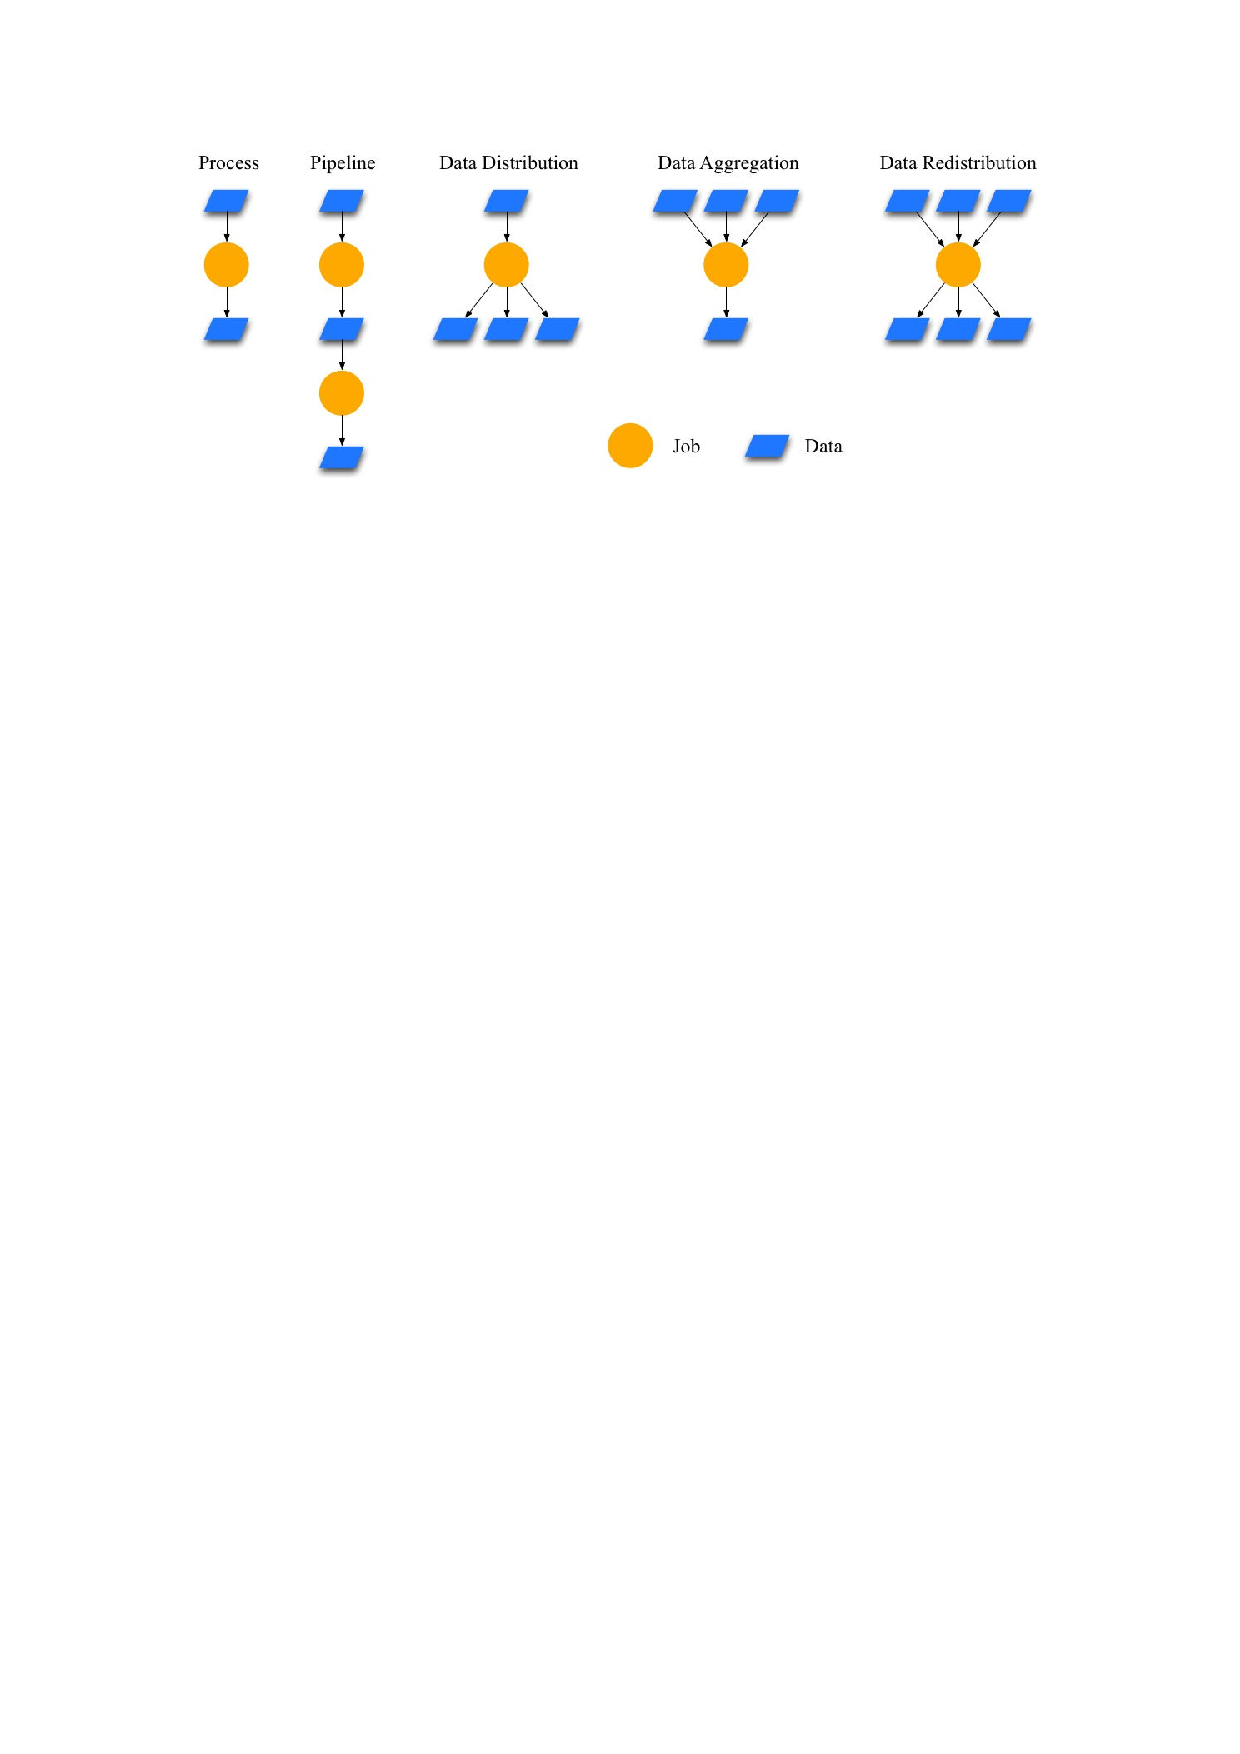
\includegraphics[width=\columnwidth]{WorkflowDataFlow}  
   \caption{Data flow structures in Workflows\cite{Bharathi08}}
   \label{fig:intro:workflow:structures}
\end{figure} 


\begin{figure}[tb]
   \centering
   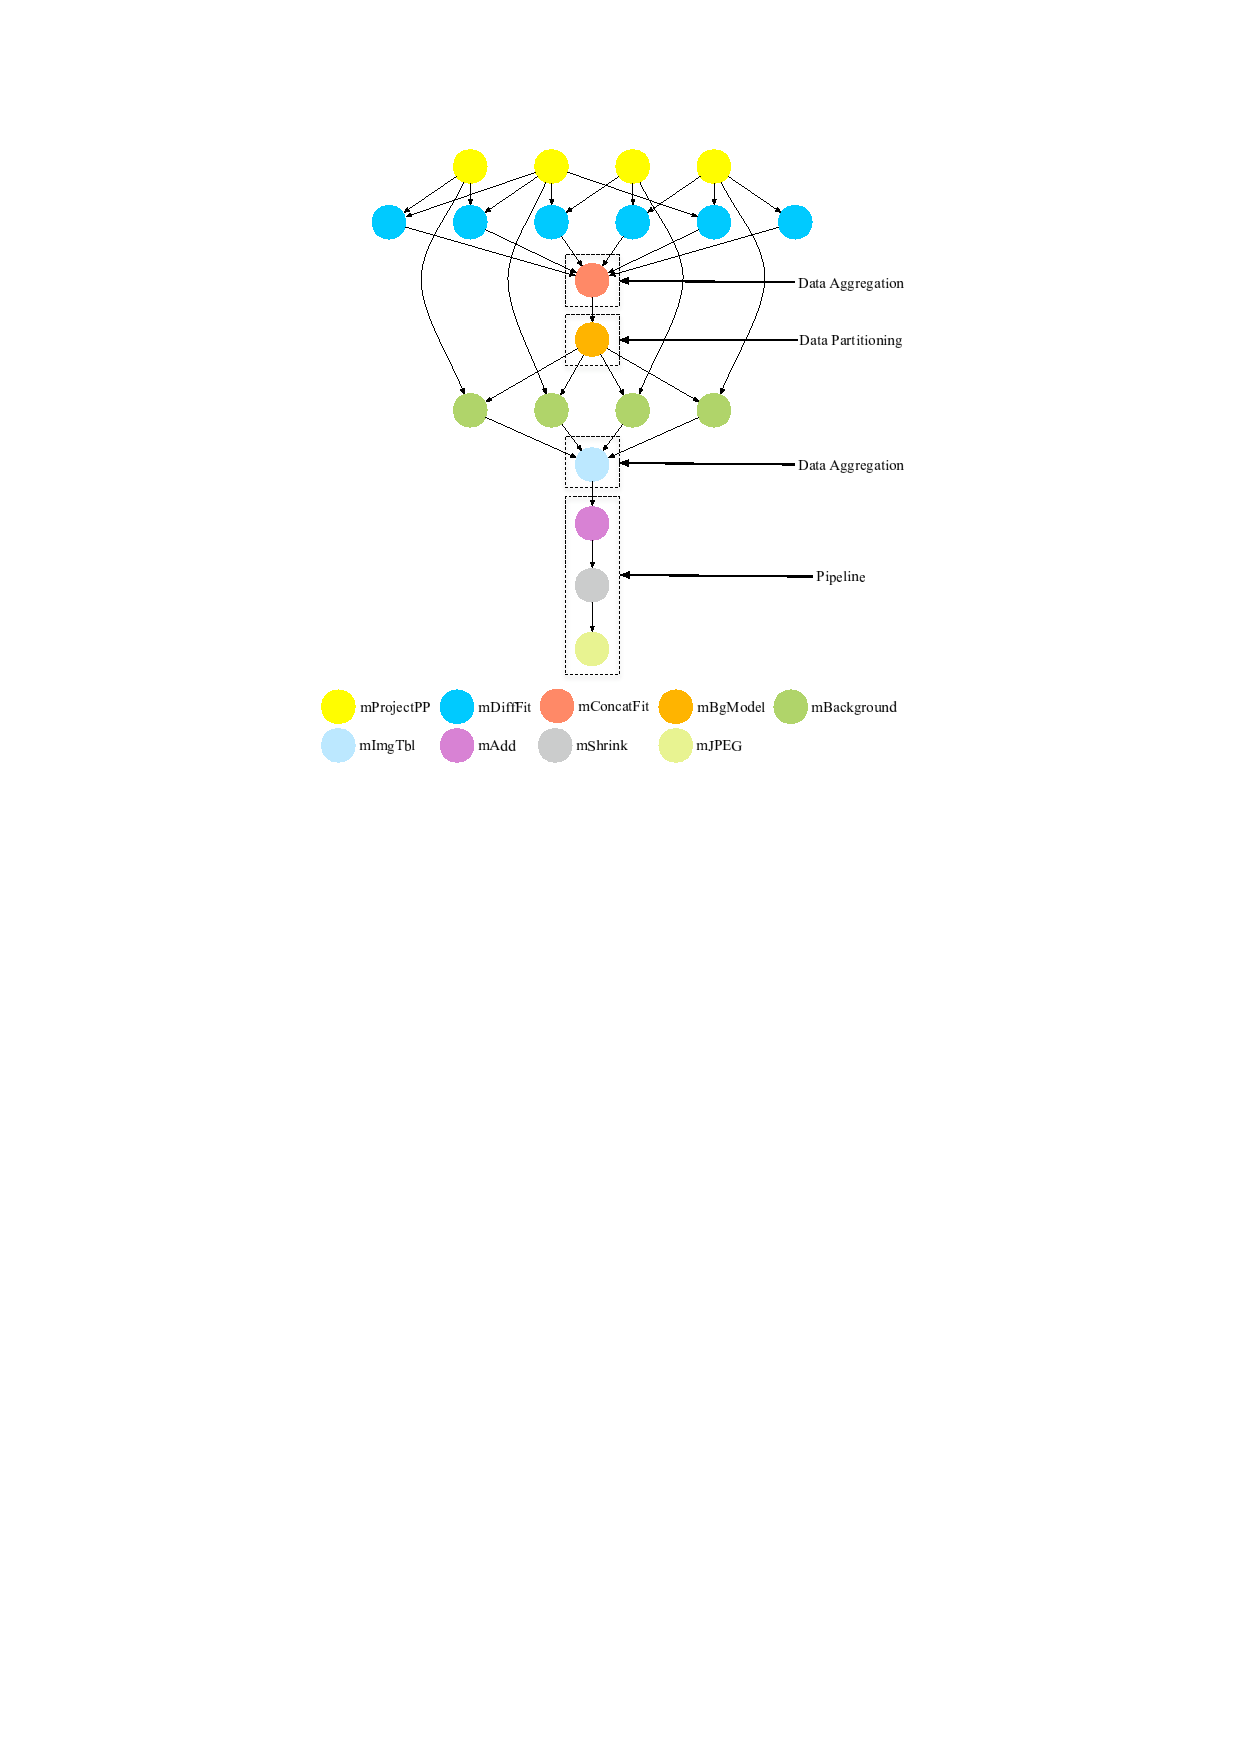
\includegraphics[width=0.7\columnwidth]{MontageWorkflow}  
   \caption{Montage – example workflow\cite{Bharathi08}}
   \label{fig:intro:workflow}\todo{Add reference to the figure in the text}
\end{figure} 

Scientific workflows are usually run on shared infrastructure as clusters, grids or clouds. It requires to carefully plan and schedule computation to efficiently use given infrastructure. As the workflows are getting bigger and more complex it is nearly impossible to do it manually. Specifically, scheduling workflow applications in a distributed system is an NP-complete problem\cite{Garey:1979:CIG:578533}. Numerous workflow algorithms to schedule workflows are presented in Chapter \ref{chap:state-of-art}.

There exist multiple workflow systems that assist scientists to create and deploy their workflow. Popular ones are Pegasus\cite{Pegasus} and Taverna\cite{Taverna}. They provide tools to model workflow either in code or via GUI application. Then one is able to generate workflow execution plan on certain (e.g. grid) architecture. Workflow systems differ in supported workflow types (DAG or non-DAG), workflow scheduling policies and algorithms, fault tolerance, and supported infrastructure. The good overview on workflow systems taxonomy is given in \cite{Yu:2005:TSW:1084805.1084814}.

\subsection{Bag of tasks}

Bag of tasks applications represent group of independent tasks that may be processed in parallel or sequentially. A large parameter sweep is good example of such problem. The \emph{map} stage of map-reduce\cite{Dean:2008:MapReduce} \todo{obrazek} application can be also considered as a bag of tasks. Additionally, many workflows include a stages of a high number parallel tasks. Such examples can be found e.g. in typical scientific workflows executed using Pegasus Workflow Management system, where e.g. CyberShake or LIGO workflows have a parallel stage of nearly homogeneous tasks~\cite{Bharathi08}. Other examples are Wien2K and ASTRO workflows that consist of iteratively executed parallel stages comprising homogeneous tasks\cite{Duan12}. Due to the high number of parallel branches, these stages accumulate the most significant computing time of the whole application, so optimization of the execution of this stage is crucial.


\section{Introduction to Cloud Computing}
\label{intro:cloud}

\todo{lepiej zaczac od tego, ze problem jest wazny i ciekawy.}Cloud computing is a jargon term without a commonly accepted non-ambiguous scientific or technical definition. The term is frequently used for marketing of hosted services or applications running in client-server model. As defined by US National Institute of Standards and Technology\cite{NISTCloudDef}, cloud computing is "a model for enabling ubiquitous, convenient, on-demand network access to a shared pool of configurable computing resources (e.g., networks, servers, storage, applications, and services) that can be rapidly provisioned and released with minimal management effort or service provider interaction".

\subsection{Service models}

We may categorize cloud services in terms of service model that give different level of control and responsibilities to user and service provider:

\begin{description}
  \item[Software as a Service (SaaS).] The capability provided to the user is to use applications deployed by provider running on a cloud infrastructure. The applications are usually available by web-browser based interface or program interface. The underlying cloud infrastructure including network, servers, operating system and application are managed by service provider. Popular SaaS applications include Gmail, Evernote and Salesforce CRM.
  \item[Platform as a Service (PaaS).] The capability provided to the user is to deploy his own appliactions created using programming languages, libraries, services and tools provied by the provider. The consumer does not manage underlying cloud infrastructure including network, servers, operating systems, runtime environment, but has control over the deployed application and configuration settings for cloud enviromnent. Example platforms include Heroku, Google App Engine and Nodejitsu.
  \item[Infrastructure as a Service (IaaS).] The capability provided to the user is to provision processing, storage, networks and other fundamental computing resources where the consumer is able to deploy and run arbitrary software. The consumer does not manage the underlying hardware infrastructure, but has control over operating system, storage, deployed appliations and has possibly limited control over networking (i.e. hosts firewall). Example platforms include Amazon EC2 and Rackspace.
\end{description}

\subsection{Deployment models}

Depending on who manages cloud infrastructure we may distinguish the following models:

\begin{description}
  \item[Private Cloud.] The cloud resources are provisioned for exclusive use by a single organization.
  \item[Community Cloud.] The cloud resources are provisioned for exclusive use by specific community of consumers from organization that have shared concerns. This is similar to scientific grid systems.
  \item[Public Cloud.] The cloud resources are provisioned for open use by the general public.
  \item[Hybrid Cloud.] The cloud infrastructure is composed of two or more distinct cloud providers that remain unique entities, but are bound together by technology that enables data and application portability. This technique is used for cloud bursting and offloading peak load to public cloud while using private resources when off-peak times.
\end{description}

\subsection{IaaS compute cloud}

Usually IaaS clouds provide three types of resources that are provisioned with a pay-per-use model: 
\begin{description}
  \item[Computing.] Provided as virtual machine (VM) instances. Multiple instance types are available that differ with CPU power, RAM memory and additional hardware (i.e. GPU units). VMs are usually billed for instance running time (wall clock time, not CPU time) usually rouned up to full hours.
  \item[Storage.] Provided as virtualized disk drives for virtual machines (i.e. Amazon's EBS) or as object store available as external service (i.e. Amazon's S3). User is usually biled for persisting data per GiB\footnote{Gibibyte $= 2^{30}$ bytes} per month. Additional charges may also apply (i.e. per IO transaction).
  \item[Networking.] Provides connectivity between VMs, storages and the Internet. User is billed for the data transfered of the cloud, while incoming data and transfer inside specific cloud usually remains free. Networking is provided in bundle with computing and storage, not as a separate service.
\end{description}

\section{Problem statement}
\label{intro:statement}

\todo{nalezy tu uzyc sformulowania 'resource allocation' zeby byc zgodnym z tytulem pracy} In this thesis we will focus on how planning and scheduling of bag of tasks and workflow applications. Planning scientific experiments requires optimization decisions that take into account both execution time and cost, as well as external constraints. Specifically, we will address the cost optimization problem of large-scale applications running on multiple heterogeneous clouds, using mathematical modeling with AMPL and mixed integer programming.

\section{Goals of the thesis}
\label{intro:goals}

The major goal of this thesis is the theoretical and practical investigation of optimization of resource allocation on the cloud by using integer linear programming tools and methods. In particular we are concerned with the following questions:

\begin{itemize}
  \item 
  \item Is it possible to perform such optimization by using AMPL?
  \item If so, is the optimization process fast enough and stable?
\end{itemize}

\todo{Dodac sekcje ``Goals of the thesis'' gdzie bedzie wypunktowana lista celow: analiza problemu, opracowania modelu, testy, itp. Pozniej w ostatnim rozdziale powinna byc ta sama lista i przy kazdym punkcie wyjasnione w jaki sposob cele zostaly zrealizowane.}

\chapter{State of the art review} \label{chap:state-of-art}  \lhead{Chapter 2. \emph{State of Art}}
 
Cloud computing is widely adopted standard for deploying web applications. Cloud users are charged on \emph{pay as you go} basis that enables for cost and service quality optimization by dynamic application scaling. Traditionally, in parallel and distributed systems like clusters and grids, workflow scheduling has been aimed to optimize the makespan or the time of completing all tasks~\cite{HEFT}. However, in context of cloud computing, the user needs to take care not only about makespan, but also about the financial cost of deploying application. Therefore, resource allocation on the cloud becomes a multi-objective optimization problem where no single optimal solution exists.

The problem of resource provisioning in IaaS clouds has been recently addressed in~\cite{Chen2011, Kim2011} and~\cite{SqueezingOut}. They typically consider unpredictable dynamic workloads and optimize the objectives such as cost, runtime or utility function by autoscaling the resource pool at runtime. In~\cite{Chen2011} they address semi-online resource provisioning for processing tasks with dynamic cloud pricing where users bid for the resources (e.g. Amazon EC2 Spot Instances).  On the other hand in~\cite{Kim2011} they consider workload offloading to the cloud from grid resources under deadline or budget constraint. In~\cite{SqueezingOut} they evaluate utility-based policy and reactive policies for dynamic resource provisioning. These approaches, however, do not address the problem of data transfer time and cost, which are an important factor when deploying scientific applications.

Automatic cloud scaling and provisioning is often delivered as a cloud service i.e. Amazon Auto Scaling\footnote{http://aws.amazon.com/autoscaling/}. Policy or rule based services are primarily designed to scale web applications~\cite{SqueezingOut} or bag of tasks applications (e.g.~\cite{ElasticSite, Kim2011}). They take input from monitoring systems and perform scaling-up or scaling-down depending on data from monitoring system. This approach is reasonable for applications with dynamic, unpredictable load as it allows to keep number of instances low, but high enough to provide certain service quality e.g. ensure acceptable request processing time.

The work presented in this thesis is related to heuristic algorithms for workflow scheduling on IaaS clouds, such as the ones described in~\cite{Abrishami2013158,Mao11,BarrionuevoFP12,BittencourtM11}. In~\cite{Abrishami2013158} the model assumes that infrastructure is provided by only one provider. In contrast, this work presents optimization on hybrid, multi-provider cloud. Infrastructure model considered differs in that we assume multiple heterogeneous clouds with object storage attached to them, instead of individual machines with peer-to-peer data transfers between them. Instead of scheduling each task individually, this approach proposes a global optimization of placement of workflow tasks and data.

Integer programming approach has been applied to the optimization of service selection for activities of QoS aware grid workflows~\cite{Brandic08}. On the other hand, in model presented in this thesis assumes the IaaS cloud infrastructure, while the objective function takes into account costs and delays of data transfers associated with the tasks.

The cost minimization problem on clouds addressed in~\cite{Pandey2010} uses a different model from ours. We impose a deadline constraint and assume that the number of instances available from providers may be limited. To satisfy these constraints, the planner has to choose resources from multiple providers. Our model also assumes that VM instances are billed per hour of usage.

The model presented in~\cite{Genez2012} also uses AMPL/CPLEX as solving platform and they define model for deadline-constrained workflow cost optimization. However, their approach does not address the problem of data transfer time and cost. Furthermore, they do not consider that number of instances on the cloud is usually limited. 

Pipelined workflows consisting of stages are addressed in~\cite{TolosanaCalasanz20121300}, where the processing model is a data flow and multiple instances of the same workflow are executed on the same set of cloud resources. The goal of this work is cost optimization instead of meeting the QoS constraints.

The deadline-constrained cost optimization of scientific workloads on heterogeneous IaaS described in~\cite{VandenBossche2013973} addresses multiple providers and data transfers between them, where the application is a bag of tasks.

\section{Summary}

None of the solutions presented in this chapter solves the problem we stated in Chapter~\ref{chap:introduction}. They solve other problems such as scheduling on only one cloud platform, or they are missing important parts of cost estimation (e.g. data transfer cost). So that, the problem of resource allocation on hybrid cloud platforms is still open. 
\chapter{Mathematical programming using AMPL}
\label{chap:ampl} 
\lhead{Chapter \ref{chap:ampl}. \emph{Mathematical programming using AMPL}}

Section \ref{sec:ampl:mathprog} presents overview on mathematical programming and problem classification (Section \ref{sec:ampl:classification}). In section \ref{sec:ampl:ampl} AMPL and other tools for mathematical programming are introduced. Then in Section \ref{sec:ampl:whiskas} we formulate example models: linear \emph{Whiskas Cat Food Problem} and integer \emph{shift work scheduling}.

\section{Mathematical Programming}
\label{sec:ampl:mathprog}

Nowdays, the term programming\cite{Programming} means writing software, but in 1940s this word was used to describe planning and scheduling activities. It appeared then that restrictions in the planning or scheduling problem may be represented mathematically using equalities and inequalities.  The solution satysfying all these constraints would be considered as acceptable plan or schedule.  Mathematical programming enables us to formally define optimization problem: it's varialbes, objective and constraints.

Defining the problem is not an easy task. If there are too few constraints, the space of possible solutions is too big. On the other hand, too many constraints can rule desirable solutions out. In the worst case there are no solutions at all. The success of programming relies on key insight into the optimized domain and modelling techniques to find a way round the possible difficulty. 

In addition to the constraints, one can define the objective --- function of the variables that makes it possible to compare solutions and select the best one. It doesn't matter how many solutions satisfy the constraints --- we are interested in the one that minimizes or maximizes the objective.

In development of optimization model it is very important to classify the problem, so we can select the most suitable way of solving it. If constraints and objectives are linear combinations of the variables then the model is called \emph{linear program} and the process of modelling and solving is called \emph{linear programming}. This class of optimization problems is particurarly important becasue a lot of real world optimization problems may be represented in such way. Additionally, there exists a lot of theory and algorithms to solve such problems in fast, deterministic way even if they have thousands of variables. The ideas of linear programming are also important for analyzing and solving problems that are non-linear.

All useful methods of mathematical programming involve using computers. The first computional method of solving optimization problems, the simplex algorithm, was introduced at that time and was subject to several improvements over the decades.

\section{Problem classification}
\label{sec:ampl:classification}

In spite of the broad applications of linear programming, the linearity assumption is too unrealistic to be applied to many of real problems. If instead smooth non-linear functions of the variables are used in constraints and objectives we call the program as \emph{non-linear program}. Solving such problems is much harder, but not impossible.

There is also another class of problems called \emph{integer programming} that assumes that variables are integer and in general it is much harder than previous. Fortuanetly, computational power of computers is still increasing and there are efficient algorithms to deal with them.

The optimization problems may be categorized in the following groups:
\begin{description}
  \item[Linear programming (LP)] Objective and constraints in this class are linear functions. Problems in this groups are usually solved by using \emph{simplex}, \emph{interior} or \emph{barrier} method.
  \item[Quadratic programming (QP)] Convex or concave objective and linear constraints. Solved by simplex-type or interior-type method.
  \item[Non-linear programming (NLP)] Continuous, but not all-linear objective and constraints. May be solved by several methods including gradient, quasi-newton, augmented lagrangian and interior-point. Unless special conditions are met, solution found is possibly optimal over only some local neighbourhood. If objective is convex (if minimized) or concave (if maximized) and constraints define a convex region it is guaranteed that optimum found is optimal over the entire feasible region.
  \item[Mixed-integer programming (MIP)] Linear objective and constraints, some or all of variables are integer-valued. Solved by branch-and-bound approach that uses a linear solver to solve subproblems.
  \item[Mixed-integer non-linear programming (MINLP)] Non-linear objective and constraints, some or all of variables are integer-valued. Solved by branch-and-bound approach that uses a non-linear solver to solve subproblems.
  \item[Constraint programming (CP)] \emph{TODO: pisac o tym w ogole?}\todo{tak :)}
\end{description}

\section{AMPL: A Mathematical Programming Language}
\label{sec:ampl:ampl}

To successfully solve optimization problem one needs to do a sequence of multiple tasks as follows:

\begin{enumerate}
  \item Formulate an abstract model: define variables, constraints and objective.
  \item Collect the data for a specific problem instance.
  \item Generate instance-specific variables, constraints and objective.
  \item Solve the problem by running a program called solver that implements algorithm that finds optimal solution.
  \item Analyze the results.
  \item Refine the model and the data as necessary, and repeat.
\end{enumerate}

Unfortuanetly, usually people use diffrent form of representing the data than algorithms do. This makes formulation and generation phases complex as modeller would like to express constraints in human-readable language e.g. mathematical notation, and solvers require to provide multiple matrices as input. We need to transform \emph{modeller's form} to \emph{algorithm's form}. Doing it manually is time consuming and erron-prone task.

To automate this task matrix generators were created for specific models. Altough they successfully automate matrix generation they are hard to code, debug and maintain. Modeller needs to be both mathematician and programmer. The other way to solve that problem is to use mathematical modelling language. Several languages\footnote{i.e. AMPL\cite{Fourer2002}, Gams\cite{Gams}, PuLP\cite{PuLP}, OscaR\cite{OscaR}} were created over the decades. 

By using modelling language, modeller may express in comfortable way also designed to serve as input for the computer. Then matrix generation may be fully automated without intermediate state of computer programming, thus mathematical programming becomes cheaper and more reliable. Benefits of formulating in modelling languages become particuraly advantageous for models being developed and subject to change.

AMPL is an algebraic mathematical modelling lanuage that resembles traditional mathematical notation to describe variables, objectives and constraints. Code in AMPL will be familiar for anybody that studied basic algebra or calculus, so that he or she doesn't need to be programmer (in present meaning). Algebraic modelling languages allow to express a wide range of optimization problems: linear, nonlinear and integer.

\subsection{Available solvers}

As soon as model is formulated and matrices generated, we may proceed with solving the specific instance of our problem. To do that we will need solver -- a program that implements one of solving algorithms. There is wide range of existing solvers available, both open-source (i.e. Cbc\cite{cbc-solver}) and commercial (i.e. CPLEX\cite{cplex}) ones that differ with the problem classes they target. Full list of available solvers is published at AMPL website\cite{AMPLSolvers}.

Usually solvers provide multiple options that let us tune them for the specific application. One may enable or disable certain features of the solver, i.e. for \emph{Bonmin}\cite{Bonmin} solver we may choose branching algorithm or configure it to use heuristics.

\section{Example -- Whiskas Cat Food Problem}
\label{sec:ampl:whiskas}
% zaczerpniete mocno z http://twiki.esc.auckland.ac.nz/twiki/bin/view/OpsRes/WhiskasCatFoodProblem

To get some practise with modelling, we will describe a typical linear programming problem on the example of Whiskas Cat Food problem. This is typical planning problem that may be found in many textbooks~\cite{dantzig}. \todo{Add non-breaking space (tilde) to all citations} The company producing the food wants to produce it as cheaply as possible while ensuring they meet the stated nutritional analysis requirements stated on the cans. 

Main ingredients of the cat food used are chicken, beef, mutton, rice wheat and gel. The prices for the ingredients are presented in Table \ref{ampl:whiskas:prices}, while ingredient contribution to the total weight of protein, fat, fibre and salt in the final product are give in Table \ref{ampl:whiskas:contribution} and nutritional requirements are presented in Table \ref{ampl:whiskas:analysis}. Given that data we may proceed with model formulation.

\begin{table}
  \centering
  \begin{tabular}{| l | r |}
    \hline
    \textbf{Ingredient} & \textbf{Price per gram} \\ \hline
    Chicken & \$ 0.013 \\ \hline
    Beef & \$ 0.008 \\ \hline
    Mutton & \$ 0.010 \\ \hline
    Rice & \$ 0.002 \\ \hline
    Wheat & \$ 0.005 \\ \hline
    Gel & \$ 0.001 \\ \hline
  \end{tabular}
  \caption{Cat food ingredient's pricing.}
  \label{ampl:whiskas:prices}  
\end{table}

\begin{table}
  \centering
  \begin{tabular}{| l | r | r | r | r |}
    \hline
    & \textbf{Protein} & \textbf{Fat} & \textbf{Fibre} & \textbf{Salt} \\ \hline
    \textbf{Chicken} & 0.100 & 0.080 & 0.001 & 0.002 \\ \hline
    \textbf{Beef} & 0.200 & 0.100 & 0.005 & 0.005 \\ \hline
    \textbf{Mutton} & 0.150 & 0.110 & 0.003 & 0.007 \\ \hline
    \textbf{Rice} & 0.000 & 0.010 & 0.100 & 0.002 \\ \hline
    \textbf{Wheat bran} & 0.040 & 0.010 & 0.150 & 0.008 \\ \hline
    \textbf{Gel} & -- & -- & -- & -- \\ \hline
  \end{tabular}
  \caption{Ingredient contribution to the final product in grams per gram of ingredient.}
  \label{ampl:whiskas:contribution}  
\end{table}

\begin{table}
  \centering
  \begin{tabular}{| l | r |}
    \hline
    Minimum \% Crude Protein & 8.0 \\ \hline
    Minimum \% Crude Fat & 6.0 \\ \hline
    Maximum \% Crude Fibre & 2.0 \\ \hline
    Maximum \% Salt & 0.4 \\ \hline
  \end{tabular}
  \caption{Cat food nutritional analysis.}
  \label{ampl:whiskas:analysis}  
\end{table}


  
\subsection{Problem formulation}

In this particular problem data defines the following data sets:

\begin{itemize}
  \item $I = \left\{\text{chicken}, \text{beef}, \text{mutton}, \text{rice}, \text{wheat}, \text{gel}\right\}$ -- defines possible ingredients,
  \item $C = \left\{\text{protein}, \text{fat}, \text{fibre}, \text{salt}\right\}$ -- defines components of nutrition.
\end{itemize}

We have also some numbers that describe members of sets;
\begin{itemize}
  \item $p_i$ -- price of given ingredient $i$ in \$ per gram
  \item $c_i,c$ -- contribution of ingredient $i$ to component of nutrition $c$ in grams per gram of ingredient.
\end{itemize}

\paragraph{Identify the decision variables}

First of all we need to identify decision variables. For the Whishas Cat Food Problem the descisions are the amounts of each ingredient we put in the can. Formally we could write this as:
\begin{align} 
  x_i &= \text{ amount (g) of ingredient $i$  in a can of cat food}
\end{align} 

\paragraph{Formulate the Objective Function}

The objective for this problem is to minimize the total cost of ingredients per fan of cat food. We know the cost per gram of each ingredient and the amount is to be found.

\begin{align}
   \min \mathop\sum\limits_{i \in I} p_i x_i
\end{align}

\paragraph{Formulate the constraints}

The constraints for the Whiskas Cat Food are:

\begin{enumerate}
  \item The sum of the amounts must make up the whole can (i.e. 100 g).
  \item The stated nutritional analysis requirements are met.
\end{enumerate}

First of the constraints can is: 

\begin{align}
   \mathop\sum\limits_{i \in I} x_i = 100
\end{align}

The latter can be written as follows

\begin{align}
   \mathop\sum\limits_{i \in I} c_{i,protein} x_i \geq 8.0 \\
   \mathop\sum\limits_{i \in I} c_{i,fat} x_i \geq 6.0 \\
   \mathop\sum\limits_{i \in I} c_{i,fibre} x_i \geq 2.0 \\ 
   \mathop\sum\limits_{i \in I} c_{i,salt} x_i \leq 0.4 \\
\end{align}

or in more general way, we may define lower and upper bounds for each component of nutrition as $L_c$ and $U_c$, the values are presented in Table \ref{ampl:whiskas:bounds}. Constraint will be written as

\begin{align}
   \mathop\forall\limits_{c \in C} L_c \leq \mathop\sum\limits_{i \in I} c_{i,c} x_i \leq U_c \\
\end{align}

\begin{table}
  \centering
  \begin{tabular}{| l | r | r |}
    \hline
    \textbf{Component of nutrition} & \textbf{Lower bound} & \textbf{Upper bound} \\ \hline
    Protein & 8.0 & -- \\ \hline
    Fat & 6.0 & -- \\ \hline
    Fibre & 2.0 & -- \\ \hline
    Salt & -- & 0.4 \\ \hline
  \end{tabular}
  \caption{Bounds for contribution of component of nutrition in percent.}
  \label{ampl:whiskas:bounds}  
\end{table}



We have formulated general problem using mathematical notation. Now we will proceed with model problem formulation using AMPL.

\subsection{Problem formulation using AMPL}

AMPL enables us to separate model definition and instance specific data. Usually we create three files: model, data and calling script. In the model file we define the data we need to have: sets and parameters, objective and constraints. Then in data file we populate the sets and parameters with the numbers for the particular instance of the problem. Both model and data files are loaded from calling script that may do some pre or post processing.

\paragraph{Model formulation}

First of all, we should define the sets for the ingredients and components of nutrition. We create file called \texttt{whiskas.mod} that will contain abstract model of optimization: sets, parameters, constraints and objective.

\begin{lstlisting}
set INGREDIENTS;
set COMPONENTS;
\end{lstlisting}

Using sets we can define the decision variables
\begin{lstlisting}
var Amount {INGREDIENTS} >= 0;
\end{lstlisting}

and parameters for the costs, components of nutrition contribution, restrictions and can size.

\begin{lstlisting}
param Cost {INGREDIENTS} >= 0;
param Contribution {INGREDIENTS, COMPONENTS} >= 0;

param Lower {COMPONENTS} default -Infinity;
param Upper {c in COMPONENTS} >= Lower[c], default Infinity;

param CanSize >= 0;

\end{lstlisting}

and the objective function

\begin{lstlisting}
minimize TotalCost : sum {i in INGREDIENTS} Cost[i] * Amount[i];
\end{lstlisting}

Note that, for the bounds that are not set, we assume \emph{±Infinity}. Additionally, we define that \emph{Cost} and \emph{Contribution} parameters should be non negative -- AMPL provides also verification of parameter data.


Finally, we may define constraints

\begin{lstlisting}
subject to MeetRequirements {c in COMPONENTS}:
  Lower[c] <= sum {i in INGREDIENTS} Contribution[i, c] * Amount[i] <= Upper[c];
  
subject to FullCan: 
  sum {i in INGREDIENTS} Amount[i] = CanSize;
\end{lstlisting}

\paragraph{Providing data}

Now we can provide the model with the data. To do this we create the file \texttt{whiskas.dat}.

First of all we need to provide sets we defined in previous paragraph.
\begin{lstlisting}
set INGREDIENTS := CHICKEN BEEF MUTTON RICE WHEAT GEL;
set COMPONENTS  := PROTEIN FAT FIBRE SALT;
\end{lstlisting}

Then we populate parameters with the data.
\begin{lstlisting}
param     Cost :=
  CHICKEN 0.013
  BEEF    0.008
  MUTTON  0.010
  RICE    0.002
  WHEAT   0.005
  GEL     0.001
;

param     Lower :=
  PROTEIN 8.0
  FAT     6.0
;

param     Upper :=
  FIBRE   2.0
  SALT    0.4
;

param CanSize := 100;

param Contribution :
          PROTEIN   FAT FIBRE  SALT :=
  CHICKEN   0.100 0.080 0.001 0.002 
  BEEF      0.200 0.100 0.005 0.005 
  MUTTON    0.150 0.110 0.003 0.007 
  RICE      0.000 0.010 0.100 0.002 
  WHEAT     0.040 0.010 0.150 0.008 
  GEL       0.0   0.0   0.0   0.0   
;
\end{lstlisting} 

\paragraph{Running AMPL}

Now we are ready to solve the model we formulated with AMPL. For that, let's create file called \texttt{whiskas.run}.

First of all we should reset AMPL environment in case that specific AMPL instance was solving other model before. We can do it with command \texttt{reset}. Then we load model using command \texttt{model} that takes model file name as an argument. Next, we load data file using command \texttt{data}. We also need to tell AMPL which solver we would like to be used. In our case we will use CPLEX (\texttt{option solver cplex}). Finally, we call solver and present results. The full file will look like as follows.

\begin{lstlisting}
reset;

model whiskas.mod;

data whiskas.dat;

option solver cplex;
solve;

display Amount;
\end{lstlisting}

Now we may run run AMPL and see if the model is working and if so, what is the optimal solution.

\begin{lstlisting}
% ampl whiskas.run
CPLEX 12.4.0.1: optimal solution; objective 0.52
2 dual simplex iterations (0 in phase I)
Amount [*] :=
   BEEF  60
CHICKEN   0
    GEL  40
 MUTTON   0
   RICE   0
  WHEAT   0
;
\end{lstlisting}

In that case, it appears that it is cheapest to use beef and fill the rest of the can with gel.

\section{Example -- Shift Scheduling}
\label{sec:ampl:sched}
\todo{say that it is an example of integer problem}
In this section, we will formulate AMPL model for shift scheduling problem\cite{Fourer2002}. The factory is working in three shift work schedule, operating six days a week from Monday to Saturday. On Saturday there's no third shift as it would overlap with Sunday. There's a certain number of workers required for each shift: more workers are required during first shift and less during the others. Due to work time regulations not all shift combinations of 5 day working week are possible. In the case described we already identified \todo{this was not described earlier} that there are 126 shift schedules possible. The crew wages depend on the choosen schedule. We also want to limit number of different schedules used, workers may work in teams during planned week. The problem is to minimize the cost of running factory while meeting all regulatory constraints.

\subsection{Problem formulation}

In this particular problem data defines the following data 

\begin{itemize}
  \item $S$ -- set of shifts,  
  \item $W$ -- set of acceptable schedules.
\end{itemize}

We have also some numbers that describe work planning;
\begin{itemize}
  \item $p_w$ -- pay rate at schedule $w$,
  \item $r_s$ -- number of staff required at shift $s$,
  \item $n_{min}$ -- minimal number of workers on any schedule.
\end{itemize}

\paragraph{Identify the decision variables}

We need to decide if given schedule will be used and if so, how many workers should follow it. Formally we could write this as:
\begin{align} 
  u_w &= \text{binary; schedule $w$ should be used iif 1} \\
  n_w &= \text{integer; how many workers should use schedule $w$}
\end{align} 

\paragraph{Formulate the Objective Function}

The objective for this problem is to minimize the total cost of running factory.

\begin{align}
   \min \mathop\sum\limits_{w \in W} p_w n_w
\end{align}

\paragraph{Formulate the constraints}

The constraints are:

\begin{enumerate}
  \item The stated minimal number of workers on each shift is met.
  \item Each schedule, if used at all, is used by minimal number of workers.
\end{enumerate}

First of the constraints is: 

\begin{align}
   \mathop\forall\limits_{s \in S}
     \mathop\sum\limits_{w \in W: s \in W_w} n_w \geq r_s
\end{align}

The second can be written as follows

\begin{align}
   \mathop\forall\limits_{w \in W}
     n_{min} u_w \leq n_w \\
   \mathop\forall\limits_{w \in W}
     n_w \leq \left(\max\limits_{s \in W_w} r_s\right) u_w 
\end{align}

We have formulated general problem using mathematical notation. Now we will proceed with model problem formulation using AMPL.

\subsection{Problem formulation using AMPL}

After we formulated the abstract model we implement it in AMPL by following the same procedure as in previous section. 

\paragraph{Model formulation}

First of all, we should define the sets and parameters in model file.

\begin{lstlisting}
set SHIFTS;
param Nsched;
set SCHEDS = 1..Nsched;
set SHIFT_LIST {SCHEDS} within SHIFTS;

param rate {SCHEDS} >= 0;
param required {SHIFTS} >= 0;
param least_assign >= 0;
\end{lstlisting}

Using sets we can define the decision variables
\begin{lstlisting}
var Work {SCHEDS} >= 0 integer; 
var Use {SCHEDS} >= 0 binary;
\end{lstlisting}

and the objective function

\begin{lstlisting}
minimize Total_Cost: sum {j in SCHEDS} rate[j] * Work[j];
\end{lstlisting}

Finally, we may define constraints

\begin{lstlisting}
subject to Shift_Needs {i in SHIFTS}:
  sum {j in SCHEDS: i in SHIFT_LIST[j]} Work[j] >= required[i];
subject to Least_Use1 {j in SCHEDS}: 
  least_assign * Use[j] <= Work[j];
subject to Least_Use2 {j in SCHEDS}:
  Work[j] <= (max {i in SHIFT_LIST[j]} required[i]) * Use[j];
\end{lstlisting}

\paragraph{Providing data}

Now we can provide the model with the data. We provide the data we defined in previous paragraph.

\begin{lstlisting}
set SHIFTS := Mon1 Tue1 Wed1 Thu1 Fri1 Sat1
              Mon2 Tue2 Wed2 Thu2 Fri2 Sat2
              Mon3 Tue3 Wed3 Thu3 Fri3 ;

param rate  default 1 ;

param required :=  Mon1 100  Mon2 78  Mon3 52 
                   Tue1 100  Tue2 78  Tue3 52
                   Wed1 100  Wed2 78  Wed3 52
                   Thu1 100  Thu2 78  Thu3 52
                   Fri1 100  Fri2 78  Fri3 52
                   Sat1 100  Sat2 78 ;
                   
param least_assign  := 5;
param Nsched        := 126 ;

set SHIFT_LIST[  1] := Mon1 Tue1 Wed1 Thu1 Fri1 ;
set SHIFT_LIST[  2] := Mon1 Tue1 Wed1 Thu1 Fri2 ;
........
set SHIFT_LIST[126] := Tue2 Wed2 Thu2 Fri2 Sat2 ;
\end{lstlisting} 

\paragraph{Running AMPL}

\begin{lstlisting}
reset;
option omit_zero_rows 1;
model whiskas.mod;

data whiskas.dat;

option solver cplex;
solve;

display Work;
display Total_Cost;
\end{lstlisting}

Now we are ready to run the model and get the results.

\begin{lstlisting}
% ampl sched.run
CPLEX 12.4.0.1: optimal integer solution; objective 266
136 MIP simplex iterations
23 branch-and-bound nodes
Work [*] :=
  3   7
  6  28
 16   8
 18   8
 20  12
 29   7
 37  21
 61   5
 66   5
 78  24
 82  28
 91  12
100   8
102   6
112  28
118  24
122  30
126   5
;

Total_Cost = 266
\end{lstlisting}

Given that data we may assign schedules to the specific workers.

\section{Conclusions}

This chapter presented basics of mathematical optimization. We discussed briefly history of optimiation, classification of optimization problems and introduced tools for mathematical optimization using computers. We also shown the example problems and corresponding models that may be solved using AMPL.
 
{ % Command scope

\newcommand{\INSTANCE}{I}
\newcommand{\STORAGE}{S}
\newcommand{\PROVIDER}{P}
\newcommand{\PROVIDERINSTANCES}{PI}
\newcommand{\LOCALSTORAGE}{LS}

\newcommand{\instancePrice}{p^I}
\newcommand{\ccu}{ccu}
\newcommand{\instanceTransferPriceIn}{p^{Iin}}
\newcommand{\instanceTransferPriceOut}{p^{Iout}}
\newcommand{\storageTransferPriceOut}{p^{Sout}}
\newcommand{\storageTransferPriceIn}{p^{Sin}}
\newcommand{\transferRate}{r}
\newcommand{\totalTasks}{A^{tot}}
\newcommand{\transferTime}{t^{net}}
\newcommand{\execTime}{t^x}
\newcommand{\dataSizeIn}{d^{in}}
\newcommand{\dataSizeOut}{d^{out}}
\newcommand{\requestPrice}{p^{R}}
\newcommand{\deadline}{t^D}
\newcommand{\instanceDeadline}{t^d}
\newcommand{\unitTime}{t^u}
\newcommand{\transferCost}{c^t}
\newcommand{\tasksPerDeadline}{a^d}
\newcommand{\timeQuantum}{t^q}
\newcommand{\tasksPerTimeQuantum}{a^q}
\newcommand{\providerMaxMachines}{n^{Pmax}}
\newcommand{\instanceMaxMachines}{n^{Imax}}

\newcommand{\NumberInstances}{N}
\newcommand{\TaskAssignment}{A}
\newcommand{\DataAssignment}{D}
\newcommand{\TailTaskHours}{R}
\newcommand{\HasTail}{H}

\chapter{Bag of tasks optimization}
\label{chap:bot} 
\lhead{Chapter \ref{chap:bot}. \emph{Bag of tasks optimization}}

   In this chapter we discuss optimization of scientific applications that may be represented as bag of uniform tasks tasks. The chapter is organized as follows: after defining application model in Section~\ref{sec:bot:appmodel} and infrastructure model in Section~\ref{sec:bot:cloudmodel}, we formulate the problem using AMPL by specifying the variables, parameters, constraints and optimization goals in \ref{sec:bot:problem}. Section~\ref{sec:bot:results} presents the results we obtained by applying the model to the scenarios involving multiple public and private clouds, overlapping computation and data transfers, and identifying special cases. In section~\ref{sec:bot:sensitivity} we provide a sensitivity analysis of our model and show how such analysis can be useful for potential users or computing service resellers. In section~\ref{sec:bot:dynamic} we estimate how our model behaves if the task sizes are not uniform and change dynamically.

\section{Application model}
\label{sec:bot:appmodel}

  The goal of this optimization model is to minimize the cost of processing a given number of tasks on a hybrid cloud platform, as discussed in Section.~\ref{sec:bot:cloudmodel}. We assume that tasks are independent from each other, but they have identical computational cost and require a constant amount of data transfer. 

  The assumption of homegeneous tasks can be justified by the reason that there are many examples of scientific applications (e.g. scientific workflows or large parameter sweeps) that include a stage of a high number of parallel nearly identical tasks. Such examples can be found e.g. in typical scientific workflows executed using Pegasus Workflow Management system, where e.g. CyberShake or LIGO workflows have a parallel stage of nearly homogeneous tasks~\cite{Bharathi08}. Other examples are Wien2K and ASTRO workflows that consist of iteratively executed parallel stages comprising homogeneous tasks~\cite{Duan12}. Due to the high number of parallel branches, these stages accumulate the most significant computing time of the whole application, so optimization of the execution of this stage is crucial. Moreover, if the tasks are not ideally homogeneous, it is possible to approximate them using a uniform set of tasks with the mean computational cost and data sizes of the application tasks. Of course, in real execution the actual task performance may vary, so the solution obtained using our optimization method becomes only approximate of the best allocation, and the actual cost may be higher and deadline may be exceeded. In order to estimate the quality of this approximation, we evaluate the impact of dynamic task runtime and and non-uniform tasks in section~\ref{sec:bot:dynamic}. 

  Model assumes that for each task a certain amount of input data needs to be downloaded, and after it finishes, the output results need to be stored. In the case of data-intensive tasks, the transfers may contribute a significant amount of total task run time.

\section{Infrastructure model}
\label{sec:bot:cloudmodel}

Three types of cloud services are required to run scientific application on the cloud: virtual machines, storage and networking. Amazon S3 and Rackspace Cloud Files are good examples of storage providers, while Amazon EC2, Rackspace, GoGrid and ElasticHosts represent computational services. In addition, the optimization model proposed in this thesis includes a private cloud running on own hardware. Each cloud provider offers multiple types of virtual machine instances with different performance and price.

For each provider the number of running virtual machines may be limited.  This is mainly the case for private clouds that have a limited capacity, but also the public clouds often impose limits on the number of virtual machines. E.g. Amazon EC2 allows maximum of 20 instances and requires to request a special permission to increase that limit~\cite{AmazonEC2FAQ}. 

Most of cloud providers charge their users for each running virtual machine on an hourly basis. Some providers charge in 5-minute (i.e. CloudSigma) or 1-minute cycles (i.e. Google Compute Enginge), but it is not widespread practise yet. Additionally, users are charged for remote data transfer while local transfer inside provider's cloud is usually free. These two aspects of pricing policies may have a significant impact on the cost of completing a scientifc task.

Cloud services are characterized by their pricing and performance. Instance types are described by price per hour, relative performance and data transfer cost as presented in Table~\ref{table:intro:cloud:pricing}. To assess the relative performance of clouds it is possible to run application-specific benchmarks on all of them, or to use publicly available cloud benchmarking services, such as CloudHarmony~\cite{CloudHarmony}. CloudHarmony defines performance of cloud instances in the units named CloudHarmony Compute Units (CCU) as similar to Amazon EC2 Compute Unit (ECU), which are approximately equivalent to CPU capacity of a 1.0-1.2 GHz 2007 Opteron or 2007 Xeon processor. Storage platforms include fees for data transfer.

\begin{table}
  \centering
  \begin{tabular}{| l | r | r |}
    \hline
    \textbf{Instance type} & \textbf{Price per hour} & \textbf{Instance performance in CCU} \\ \hline
    \multicolumn{3}{|c|}{\textbf{Amazon Web Services (AWS) [US East]}}       \\ \hline
    m2.4xlarge        & \$2.400   & 27.25                                    \\ \hline
    m2.2xlarge        & \$1.200   & 14.89                                    \\ \hline
    linux.c1.xlarge   & \$0.680   & 8.78                                     \\ \hline
    m2.xlarge         & \$0.500   & 7.05                                     \\ \hline
    m1.xlarge         & \$0.680   & 5.15                                     \\ \hline
    m1.large          & \$0.340   & 4.08                                     \\ \hline
    c1.medium         & \$0.170   & 3.43                                     \\ \hline
    m1.small          & \$0.085   & 0.92                                     \\ \hline
    \multicolumn{3}{|c|}{\textbf{Rackspace Cloud [Dallas]}}                  \\ \hline
    rs-16gb           & \$0.960   & 4.95                                     \\ \hline
    rs-2gb            & \$0.120   & 4.94                                     \\ \hline  
    rs-1gb            & \$0.060   & 4.93                                     \\ \hline
    rs-4gb            & \$0.240   & 4.90                                     \\ \hline
    \multicolumn{3}{|c|}{\textbf{GoGrid [CA, US]}}                           \\ \hline
    gg-8gb            & \$1.520   & 23.2                                     \\ \hline
    gg-4gb            & \$0.760   & 9.28                                     \\ \hline
    gg-2gb            & \$0.380   & 4.87                                     \\ \hline
    gg-1gb            & \$0.190   & 4.42                                     \\ \hline
    \multicolumn{3}{|c|}{\textbf{ElasticHosts [UK]}}                         \\ \hline
    eh-8gb-20gh       & \$0.654   & 9.98                                     \\ \hline
    eh-4gb-8gh        & \$0.326   & 5.54                                     \\ \hline
    eh-2gb-4gh        & \$0.164   & 4.75                                     \\ \hline
    eh-1gb-2gh        & \$0.082   & 4.30                                     \\ \hline
    \multicolumn{3}{|c|}{\textbf{Hyphotetical instance of private cloud}}    \\ \hline
    private           & \$0.000   & 1.00                                     \\ \hline
  \end{tabular}
  \caption{Example pricing and performance of cloud instances.}
  \label{table:intro:cloud:pricing}  
\end{table}


\section{Problem formulation}
\label{sec:bot:problem}

  To perform optimization of the total cost, Mixed Integer Non-Linear Problem (MINLP) is formulated and implemented in A Mathematical Programming Language (AMPL)~\cite{Fourer2002}.  As we shown in Chapter~\ref{chap:ampl}, AMPL requires to specify input data sets and variables to define the search space, as well as constraints and objective function to be optimized.

\subsection{Input data}
 
  The formulation requires the following input sets, which represent the cloud infrastructure model:
  \begin{itemize}
      \item $\STORAGE = \{s3, cloudfiles\}$ -- defines available cloud storage
      sites,
      \item $\PROVIDER = \{amazon, rackspace, \dotsc\}$ -- defines
      possible computing cloud providers,
      \item $\INSTANCE = \{m1.small, \dots, gg.1gb, \dotsc\}$ -- defines
      instance types,
      \item $\PROVIDERINSTANCES_{p} \subset \INSTANCE$ -- instances that
      belong to provider $\PROVIDER_p$,
      \item $\LOCALSTORAGE_{s} \subset \PROVIDER$ -- compute cloud providers
      that are local to storage platform $\STORAGE_s$.
  \end{itemize}        
    
  Each instance type $\INSTANCE_i$ is described by the following parameters:
  \begin{itemize}
      \item $\instancePrice_i$ -- fee in \$ for running instance $\INSTANCE_i$
      for one hour,
      \item $\ccu_i$ -- performance of instance in CloudHarmony Compute Units
      (CCU),
      \item $\instanceTransferPriceOut_i$ and $\instanceTransferPriceIn_i$ --
      price for non-local data transfer to and from the instance, in \$ per
      MiB.
  \end{itemize}

  Storage sites are characterized by:
  \begin{itemize}
      \item $\storageTransferPriceOut_s$ and $\storageTransferPriceIn_s$
      characterize price in \$ per MiB for non local data transfer.
  \end{itemize}

  Additionally, we need to provide data transfer rates in MiB per second between storage and instances by defining function $\transferRate_{i,s} > 0$ .

  We assume that the computation time of a task is known and constant, this also applies to input and output data size. We also assume that tasks are atomic (non divisible). Computation is characterized by the following parameters:
  \begin{itemize}
      \item $\totalTasks$ -- number of tasks,
      \item $\execTime$ -- execution time in hours of one task on 1 CCU
      machine,
      \item $\dataSizeIn$ and $\dataSizeOut$ -- data size for input and
      output of one task in MiB,
      \item $\requestPrice$ -- price per request for queuing service,
      \item $\deadline$ -- total time for completing all tasks in hours (deadline).
  \end{itemize} 

\subsection{Auxiliary parameters}

  The formulation of the problem requires a set of precomputed parameters which are derived from the main input parameters of the model. The relevant  parameters include:
  \begin{align}
      \transferTime_{i,s} &= \frac{\dataSizeIn+\dataSizeOut}{\transferRate_{i,s} \cdot 3600}  \\
      \label{bot:unitTime}\unitTime_{i,s} &= \frac{\execTime}{\ccu_i} + \transferTime_{i,s}  \\
      \transferCost_{i,s} &= (\dataSizeOut \cdot (\instanceTransferPriceOut_i + \storageTransferPriceIn_s) + \dataSizeIn \cdot (\storageTransferPriceOut_s+\instanceTransferPriceIn_i)) \\
      \label{bot:tasksPerDeadline}\tasksPerDeadline_{i,s} &= \lfloor\frac{\deadline}{\unitTime_{i,s}}\rfloor \\
      \timeQuantum_{i,s} &= \lceil \unitTime_{i,s} \rceil \\
      \tasksPerTimeQuantum_{i,s} &= \lfloor\frac{\timeQuantum_{i,s}}{\unitTime_{i,s}}\rfloor \\
      \label{bot:instanceDeadline}\instanceDeadline_{i,s} &= \lceil\lfloor\frac{\deadline}{\unitTime_{i,s}} \rfloor \cdot \unitTime_{i,s} \rceil
  \end{align}
  \begin{itemize}
      \item $\transferTime_{i,s}$ -- {\em transfer time}: time for data transfer between
      $\INSTANCE_i$ and $\STORAGE_s$,
      \item $\unitTime_{i,s}$ -- {\em unit time}: time for processing a task
      on instance $\INSTANCE_i$ using storage $\STORAGE_s$ that includes computing and
      data transfer time (in hours),
      \item $\transferCost_{i,s}$ -- cost of data transfer between instance
      $\INSTANCE_i$ and storage $\STORAGE_s$,
      \item $\tasksPerDeadline_{i,s}$ -- number of tasks that can be done on
      one instance $\INSTANCE_i$ when using storage $\STORAGE_s$ running for $\deadline$ hours,
      \item $\timeQuantum_{i,s}$ -- {\em time quantum}: minimal increase of
      instance running time that is sufficient to increase the number of
      processed tasks, rounded up to full hour,
      \item $\tasksPerTimeQuantum_{i,s}$ -- number of tasks that can be done
      in $\timeQuantum_{i,s}$ hours,
      \item $\instanceDeadline_{i,s}$ -- {\em instance deadline}: number of
      hours that can be effectively used for computation.
  \end{itemize}

\subsection{Variables}
\label{sec:bot:varialbes}
  Variables that will be optimized and define the solution space are listed below:
  \begin{itemize}
      \item $\NumberInstances_i$ -- number of instances of type $\INSTANCE_i$
      to be deployed,
      \item $\TaskAssignment_i$ -- number of tasks to be processed on
      instances of type $\INSTANCE_i$,
      \item $\DataAssignment_s$ -- $1$ iif $\STORAGE_s$ is used, otherwise $0$; only one storage may be used,
      \item $\TailTaskHours_i$ -- number of remainder (tail) hours for
      instance $\INSTANCE_i$,
      \item $\HasTail_i$ -- $1$ iif $\TailTaskHours_i \neq 0$, otherwise $0$.
  \end{itemize}


  Fig.~\ref{fig:bot:policy} illustrates how the tasks are assigned to multiple running instances. The tasks are atomic and there is no checkpointing or preemption. Even though all the tasks have the same computational cost, their total processing time depends on performance of the VM type and data transfer rate. Moreover, the users are charged for the runtime of each VM rounded up to full hours. In our model the tasks are assigned to the instances in the following way. First, in the process of optimization $\TaskAssignment_i$ tasks are assigned to the instance $\INSTANCE_i$. This gives $\NumberInstances_i$  instances of type $\INSTANCE_i$ running for $\instanceDeadline_{i,s}$ hours. Remaining tasks are assigned to an additional instance running for $\TailTaskHours_i$ hours. We will refer to them as tail hours.

  \begin{figure}[tb] 
     \centering
     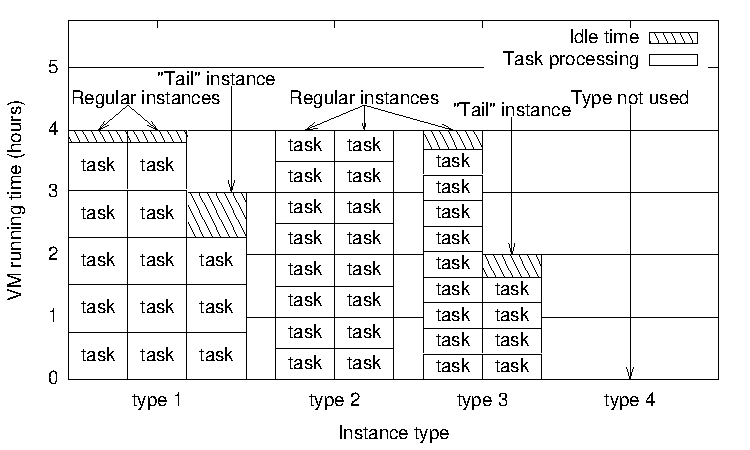
\includegraphics[width=0.7\columnwidth]{BagOfTasks/scheduling_policy.pdf}
     \caption{\label{fig:bot:policy}Task scheduling policy}
  \end{figure}
    

  In order to enforce provider's instance limit, $\HasTail_i$ is introduced which indicates if $\INSTANCE_i$ has any tail hours. E.g. in Fig.~\ref{fig:bot:policy} instances of type 1 have 3 tail hours, and instances of type 2 have no tail hours.


\subsection{Formulation of constraints and objectives}

  Cost of running a single task which includes the cost of VM instance time required for data transfer and task computing time, together with data transfer costs and request cost, can be described as: 

  \begin{align*}
      \left(\transferTime + \unitTime\right) \cdot \instancePrice + \\
      \dataSizeIn \cdot \left(\storageTransferPriceOut + \instanceTransferPriceIn\right) + \\
      \dataSizeOut \cdot \left(\instanceTransferPriceOut + \storageTransferPriceIn\right) + \\
      \requestPrice
  \end{align*}

  The objective function represents the total cost of running multiple tasks of the application on the cloud infrastructure and it is defined as:

  \begin{align}    
      \underset{\text{total cost}}{\text{minimize}} \sum \limits_{i \in \INSTANCE}  ( & 
                   (\sum\limits_{s \in \STORAGE} \DataAssignment_s\cdot\instanceDeadline_{i,s}\cdot\NumberInstances_i + \TailTaskHours_i) \cdot \instancePrice_i  
                    + \TaskAssignment_i\cdot(\requestPrice + \sum\limits_{s \in \STORAGE} \DataAssignment_s \cdot \transferCost_{i,s})
                 )
  \end{align}
  
  subject to the constraints:
  \nopagebreak 
  \begin{align}
     \label{bot:cSolutionConstraintsBegin}\mathop\forall\limits_{i \in \INSTANCE} & \TaskAssignment_i \in \mathbb{Z} \land 0 \leq \TaskAssignment_i \leq \totalTasks  \\
     \mathop\forall\limits_{s \in \STORAGE}  & \DataAssignment_s \in \{0, 1\} \\ 
     \mathop\forall\limits_{i \in \INSTANCE} & \NumberInstances_i \in \mathbb{Z} \land 0 \leq \NumberInstances_i \leq \instanceMaxMachines_i \\
     \mathop\forall\limits_{i \in \INSTANCE} & \TailTaskHours_i \in \mathbb{Z} \land 0 \leq \TailTaskHours_i \leq \deadline - 1 \\
     \label{bot:cSolutionConstraintsEnd}\mathop\forall\limits_{i \in \INSTANCE} & \HasTail_i \in \{0, 1\} \\
     \label{bot:cTaskAssignmentBounds}\mathop\forall\limits_{i \in \INSTANCE}
          & \TaskAssignment_i \geq \sum_{s \in \STORAGE} (\NumberInstances_i \cdot
          \tasksPerDeadline_{i,s}) \cdot \DataAssignment_s
          \\
      \label{bot:cTaskAssignmentBounds2}\mathop\forall\limits_{i \in \INSTANCE}
          & \TaskAssignment_i \leq  \sum_{s \in \STORAGE} (\NumberInstances_i \cdot
          \tasksPerDeadline_{i,s} + \max(\tasksPerDeadline_{i,s} - 1, 0)) \cdot
          \DataAssignment_s\\
     \label{bot:cTailTasksHoursBounds}\mathop\forall\limits_{i \in \INSTANCE}
          & \TailTaskHours_i \geq \sum_{s \in \STORAGE} (\TaskAssignment_i - \NumberInstances_i \cdot
          \tasksPerDeadline_{i,s}) \cdot \unitTime_{i,s} \cdot \DataAssignment_s
          \\ 
     \label{bot:cTailTasksHoursBounds2}\mathop\forall\limits_{i \in \INSTANCE}
          & \TailTaskHours_i  \leq \sum_{s \in \STORAGE} (\TaskAssignment_i -
          \NumberInstances_i \cdot \tasksPerDeadline_{i,s} +
          \tasksPerTimeQuantum_{i,s}) \cdot \unitTime_{i,s} \cdot
          \DataAssignment_s\\ 
     \label{bot:cSumTasks}& \sum\limits_{i \in \INSTANCE} \TaskAssignment_i = \totalTasks \\
     \label{bot:cData}& \sum\limits_{s \in \STORAGE} \DataAssignment_s = 1 \\ 
     \label{bot:cSetHasTailBounds}\mathop\forall\limits_{i \in \INSTANCE} &
     \HasTail_i \leq \TailTaskHours_i \leq \max(\deadline-1,0)\cdot\HasTail_i
     \\ \label{bot:cMaxMachines}\mathop\forall\limits_{p \in \PROVIDER} & \sum_{i \in \PROVIDERINSTANCES_p} (\HasTail_i + \NumberInstances_i) \leq \providerMaxMachines_p
  \end{align}

  Interpretation of the constraints is the following:
  \begin{itemize}
      \item(\ref{bot:cSolutionConstraintsBegin}) to
      (\ref{bot:cSolutionConstraintsEnd}) define weak constraints for a solution, i.e. they are to ensure that the required variables have the appropriate integer or binary values,
      \item(\ref{bot:cTaskAssignmentBounds}) and (\ref{bot:cTaskAssignmentBounds2}) ensure that number of instances is adequate to number of assigned tasks; for chosen storage $\DataAssignment_s$
      \begin{align*}
          \NumberInstances_i \cdot \tasksPerDeadline_{i,s} \leq \TaskAssignment_i \leq \NumberInstances_i \cdot \tasksPerDeadline_{i,s} + \max\left(\tasksPerDeadline_{i,s} - 1, 0\right)
      \end{align*} where the lower bound is given by full allocation of $\NumberInstances_i$ machines and the upper bound includes a fully allocated tail machine,
      \item(\ref{bot:cTailTasksHoursBounds}) and (\ref{bot:cTailTasksHoursBounds2})
      ensure that number of tail hours is adequate to number of remaining
      tasks, implement $\TailTaskHours_i = \ceil*{\left(\TaskAssignment_i - \NumberInstances_i \cdot \tasksPerDeadline_{i,s}\right) \cdot \unitTime_{i_s}}$,
      \item(\ref{bot:cSumTasks}) ensures that all tasks are processed,
      \item(\ref{bot:cData}) ensures that only one storage site is selected,
      \item(\ref{bot:cSetHasTailBounds}) ensures that $\TailTaskHours_i$ has proper value,
      implements $\HasTail_i = \left\{\begin{array}{cc} 1, & \TailTaskHours_i\; >\; 0 \\ 0, & \TailTaskHours_i\; =\; 0 \end{array}\right.$,
      \item(\ref{bot:cMaxMachines}) enforces providers' instance limits. 
  \end{itemize}

\subsection{Solver choice}

  Defining the problem in AMPL enables to choose among a wide range of solvers that can be used as backend. The problem itself is MINLP, but can be reduced to Integer Linear Programming (ILP) problem. The nonlinear part of problem comes from storage choice, so by fixing storage provider and running optmization procedure for each storage separately the optimal solution is found.

  Initially {Bonmin}~\cite{Bonami2008} solver was used, but after the model was fully implemented and subject to more tests, it appeared that CBC~\cite{cbc-solver} solver performs better with default options. This results from the fact that {Bonmin} is a solver designed to solve MINLP problems and uses various heuristics, while CBC uses a branch and bound algorithm tuned for ILP. As the problem is linear and convex, CBC finds global optimum. The model was optimized so that it should give acceptable results in $\sim$0.10 seconds \footnote{As measured on quad-core Intel i5 machine.}. 

\section{Experiments and results}
\label{sec:bot:results}
    
  To evaluate the model, I first run the optimization process for two scenarios with a private cloud and (1) infinite public clouds (Section~\ref{sec:bot:private-infinite}) and (2) finite public clouds (Section~\ref{sec:bot:private-finite}). I also evaluated the effect of possible overlapping of computations and data transfers in Section~\ref{sec:bot:overlapping}. When testing the model under various input parameters, I identified interesting special cases described in Section~\ref{sec:bot:special}. Finally, I discuss a sensitivity analysis, its implications and potential usage in Section~\ref{sec:bot:sensitivity}.
    
  Data intensive tasks that require relatively large amount of data for short computing time (we assumed 512 MiB of input and 512 MiB of output) and compute intensive tasks that require relatively small amount of data (we assumed 0.25 MiB of input and 0.25 MiB of output). Each case consists of 20,000 tasks, each of them requires 0.1 hour of computing time on a VM with performance of 1 CCU. Two scenarios with infinite and finite public clouds were considered, where as the costs and performance of public clouds we used the data from CloudHarmony benchmarks. This dataset gives the data of 4 compute cloud providers (Amazon EC2, Rackspace, ElasticHosts and GoGrid) and 2 storage providers (Amazon S3 and Rackspace Cloud Files), giving the instance prices between \$0.06 and \$2.40 per hour and performance between 0.92 and 27.4 CCU (see Table~\ref{table:intro:cloud:pricing}). The pricing model assumes that the private cloud instances have the performance of 1 CCU and \$0 cost.  For each scenario the deadline parameter ranges between 5 and 100 hours.  Since only two storage providers (S3 and Cloud Files) were considered, the solver is run separately for these two parameters.
    
\subsection{Private + infinite public clouds}
\label{sec:bot:private-infinite} 
  This scenario assumes that the private cloud can run a maximum of 10 instances, while the public clouds have unlimited capacity. The results for tasks that require small amount of data are shown in Fig.~\ref{fig:bot:small-infinite}. As the deadline is extended, the total cost linearly drops as expected. As many tasks as possible are run on the private cloud, and for all the remaining tasks the instance type with best price to performance ratio is selected.
    
  This situation changes as data size grows (Fig.~\ref{fig:bot:large-infinite}) -- for data intensive tasks the total cost is nearly constant as all the work is done on a public cloud. This results from the fact that data transfer cost to and from the private cloud is higher than the cost of running instances on public cloud. In our case it turns out that the lowest cost can be achieved when using Cloud Files storage from Rackspace, since in our dataset the best instance type in terms of price to performance was available at Rackspace. 
        
  \begin{figure}[tb] 
     \centering
     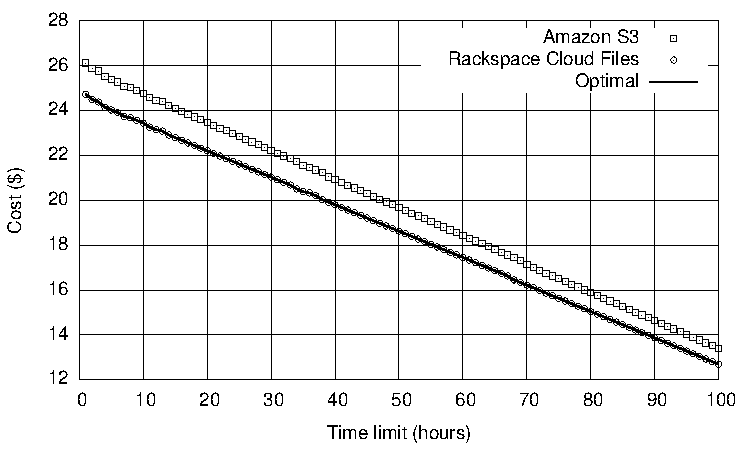
\includegraphics[width=0.7\columnwidth]{BagOfTasks/graph-small-infinite.pdf}
     \caption{Small data processed on infinite public cloud\label{fig:bot:small-infinite}}
     
  \end{figure}

  \begin{figure}[tb] 
     \centering
     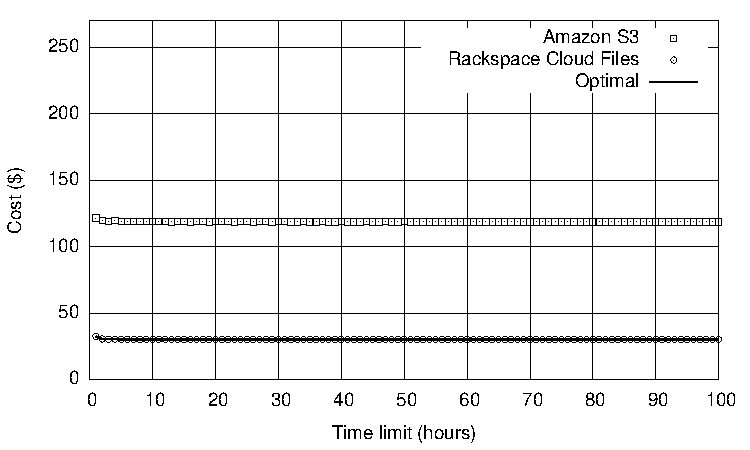
\includegraphics[width=0.7\columnwidth]{BagOfTasks/graph-large-infinite.pdf}
     \caption{Large data processed on infinite public cloud\label{fig:bot:large-infinite}}
  \end{figure}        
    
\subsection{Private + finite public clouds}
\label{sec:bot:private-finite}
    
  If assumption that public clouds are limited is made, situation is not so straightforward (See Fig.~\ref{fig:bot:small-finite} and~\ref{fig:bot:large-finite}). For relatively long deadlines, a single cloud platform for both VMs and storage can be used, which means that the data transfer is free. As the deadline shortens we first observe a linear cost increase. At the point when the selected cloud platform reaches its VM limit, additional clouds need to be used, so we need to begin paying for the data transfer. Therefore the cost begins to increase more rapidly.
  
  \begin{figure}[tb]
     \centering
     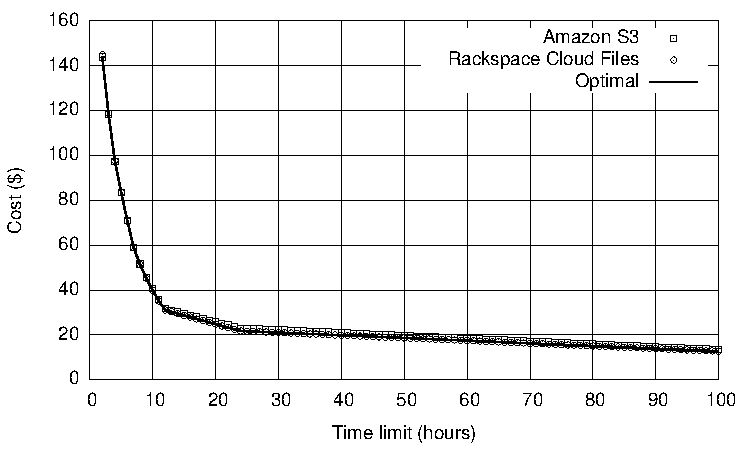
\includegraphics[width=0.7\columnwidth]{BagOfTasks/graph-small-finite.pdf}
     \caption{Small data processed on finite public
     cloud\label{fig:bot:small-finite}}
  \end{figure}

    
  This effect is very significant in the case of data intensive tasks (Fig.~\ref{fig:bot:large-finite}) as the cost growth may become very steep. For example, in our tests the task processing cost in 28 hours was \$157.39, in 30 hours it was \$131.14 and in 34 hours it was only \$30.26. For longer deadlines there was no further decrease. We can also observe that for longer deadlines the Cloud Files storage provider is less expensive for the same reason as it was in Fig.~\ref{fig:bot:large-infinite}. Shorter deadlines, however, require to run more powerful instances from other clouds (Amazon EC2), thus it becomes more economical to use its local S3 storage.
    
  \begin{figure}[tb]
     \centering
     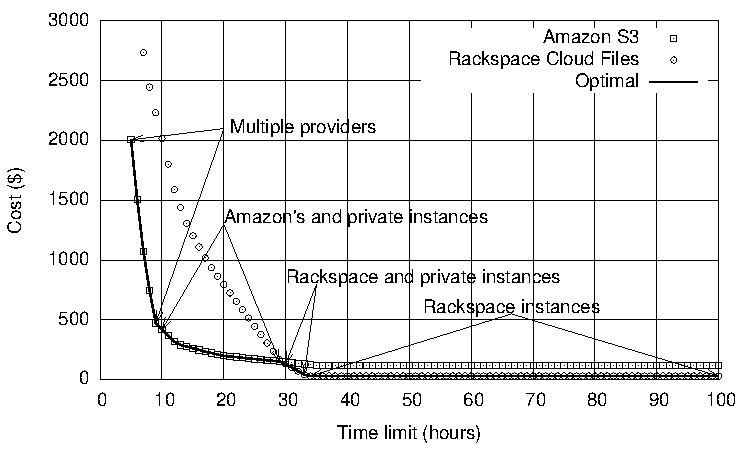
\includegraphics[width=0.7\columnwidth]{BagOfTasks/graph-large-finite.pdf}
     \caption{Large data processed on finite public
     cloud\label{fig:bot:large-finite}}
  \end{figure}  
  
\subsection{Overlapping computation and data transfers}
\label{sec:bot:overlapping}
  
  In our model we assumed that computation and data transfers are not overlapping. To achieve parallelism of these two processes, the model needs to be modified in the following way. The total task computation time is maximum of task execution and data transfer time. Additionally, input for the first task and output of the last task must be transferred sequentially. Equations \ref{bot:unitTime}, \ref{bot:tasksPerDeadline} and \ref{bot:instanceDeadline} are updated for this case as follows:
  
  \begin{align}
      \unitTime_{i,s} &= \max(\frac{\execTime}{\ccu_i}, \transferTime_{i,s})  \\    
      \tasksPerDeadline_{i,s} &= \lfloor\frac{(\deadline - \transferTime_{i,s})}{\unitTime_{i,s}}\rfloor \\         
      \instanceDeadline_{i,s} &= \lceil\lfloor\frac{(\deadline - \transferTime_{i,s})}{\unitTime_{i,s}} \rfloor \cdot \unitTime_{i,s} \rceil            
  \end{align}
  
  Fig.~\ref{fig:bot:large-finite-overlap} shows results for the same experiment as in Section~\ref{sec:bot:private-finite} and Fig.~\ref{fig:bot:large-finite}, but with computing and transfers overlapping. Overlapping reduces total cost as time required for task processing is significantly lower.  This is especially true for shorter deadlines when multiple clouds are used, as transfer rates are lower between different clouds comparing to one provider infrastructure.
  
  \begin{figure}[tb]
     \centering
     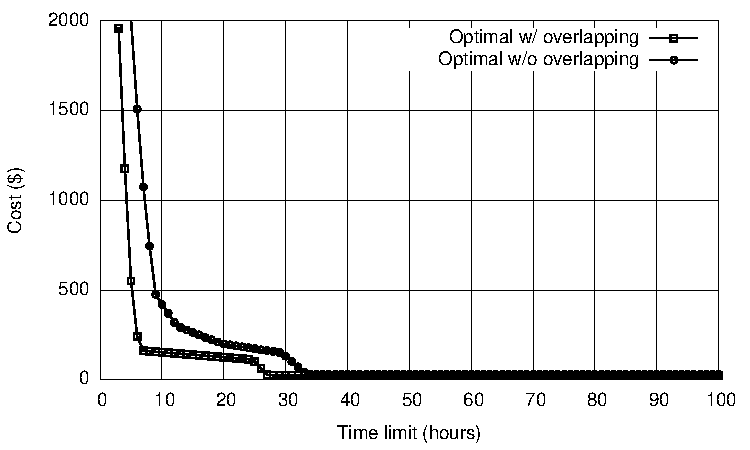
\includegraphics[width=\columnwidth]{BagOfTasks/overlap.pdf}
     \caption{Large data processed on finite public cloud with overlapping computation and data transfer\label{fig:bot:large-finite-overlap}}
  \end{figure}  

\subsection{Identifying special cases}
\label{sec:bot:special}
  
  Running a test case with very large tasks which cannot be completed within one hour on largest available instance revealed an interesting model behaviour. Results are shown on Fig.~\ref{fig:bot:special-case-results}. Local minima may occur for certain deadlines thus cost does not increase monotonically with decrease of deadline. This is a consequence of our task scheduling policy, as explained in Section~\ref{sec:bot:varialbes}. In the case of large tasks, the schedule for deadline of 9 hours  as seen in Fig.~\ref{fig:bot:special-case-009-cf} costs less than for deadline of 10 hours as in Fig.~\ref{fig:bot:special-case-010-cf}. In the first case the total number of VM-hours of the \emph{gg-8mb} instance is equal to 56, but in the case of deadline of 10 hours the total number is 58, which results in higher cost. This is the result of the policy, which tries to keep VMs running time as close to the deadline as possible. Such policy is based on general observation, that for a given budget it is usually more economical to start less VMs for longer time than to start more VMs for shorter time. However, there are rare cases when such policy may lead to non-optimal solutions. It should be noted, that the solution of the model returned by the solver in this case is optimal, but it is the model itself that does not allow to find the minimum cost.
  
  Moreover, for longer deadlines the cost is a step function -- e.g. the cost for deadline of 18 hours is the same as for 14 hours. These two observations suggest that the model could be modified in such a way that the deadline is also a variable with upper bound constraint. Similar result can be achieved in a simple way by solving the current model for multiple deadlines in the neigborhood of the desired deadline and by selecting the best solution.  
  
  \begin{figure}[tb]
     \centering 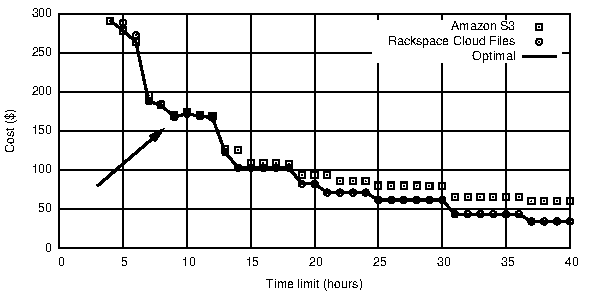
\includegraphics[width=\columnwidth]{BagOfTasks/special-case-results.pdf}
     \caption{Special case with local minimum for deadline 9
     \label{fig:bot:special-case-results}}
  \end{figure}

  \begin{figure}[tb]
     \centering  
     \begin{subfigure}[b]{0.49\textwidth}
       \centering       
       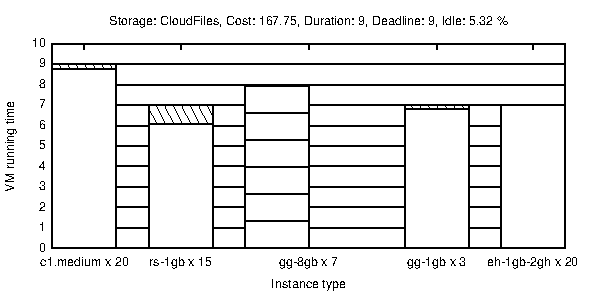
\includegraphics[width=\textwidth]{BagOfTasks/special-case-009-cf.pdf}
       \caption{Deadline = 9 hours}
       \label{fig:bot:special-case-009-cf}
     \end{subfigure}
     \begin{subfigure}[b]{0.49\textwidth}
       \centering       
       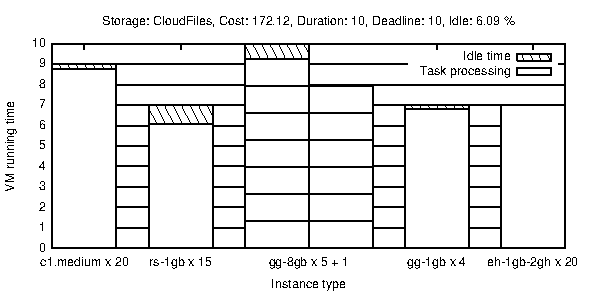
\includegraphics[width=\textwidth]{BagOfTasks/special-case-010-cf.pdf}
       \caption{Deadline = 10 hours}
       \label{fig:bot:special-case-010-cf}
     \end{subfigure}
     \caption{Task schedule for the identified special case}
  \end{figure}
    
\section{Sensitivity analysis}
\label{sec:bot:sensitivity}
    
  \begin{figure*}[tb]
     \centering 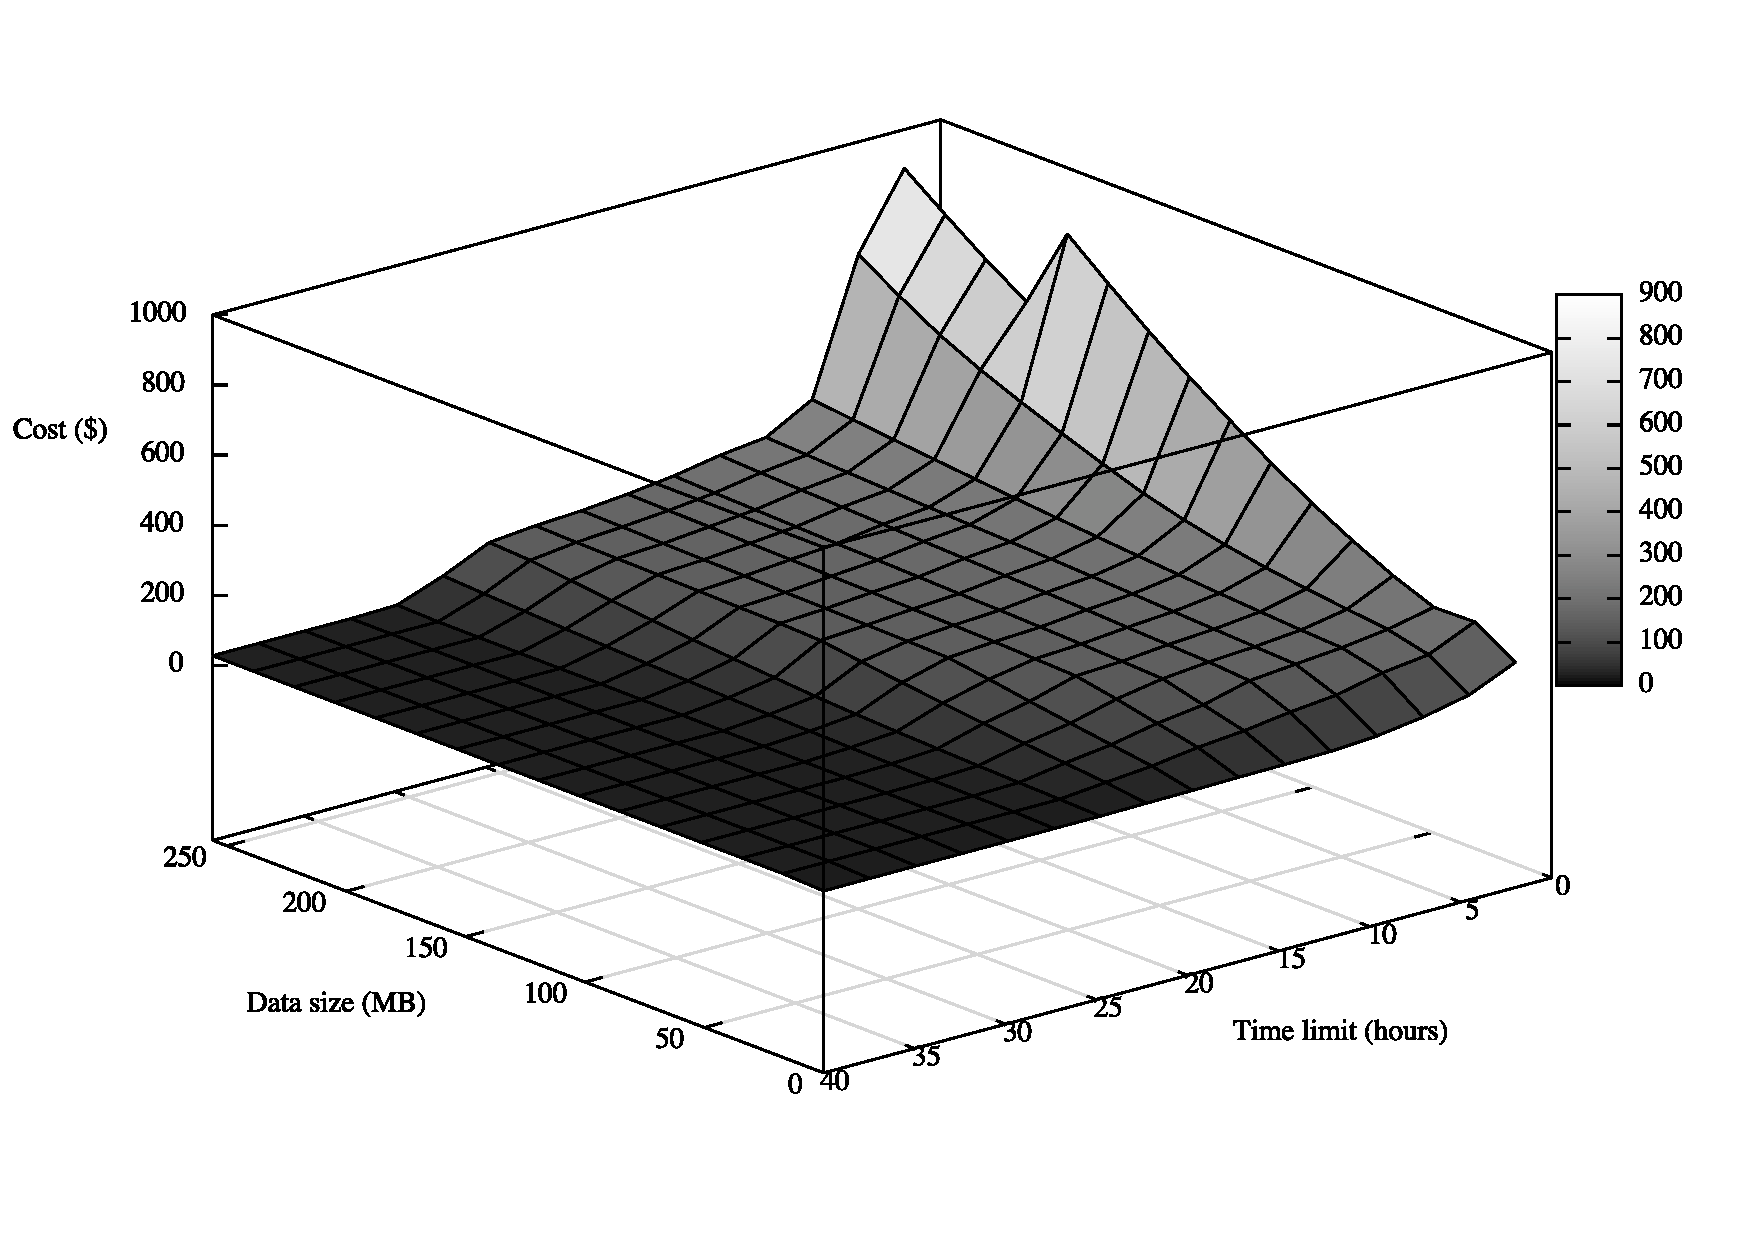
\includegraphics[width=0.7\textwidth]{BagOfTasks/sensitivity-surface}
     \caption{Optimal cost for a wide range of deadline constraints and data
     sizes.\label{fig:bot:sensitivity-surface}}
  \end{figure*} 
  
  In order to better assess how the model behaves in response to the changing
  constraints and for varying input parameters, I performed a sensitivity
  analysis by sampling a large parameter space.
  Fig. \ref{fig:bot:sensitivity-surface} shows the solutions obtained for deadlines
  ranging from 2 to 40 hours and for input and output data sizes ranging from
  0 to 256 MiB. As it can be seen in the plot, for all data sizes the cost
  increases monotonically with the decrease of the deadline, which confirms
  that no anomalies are observed. The same data can be also observed as
  animated plot available as on-line supplement\footnote{See also
  \url{http://youtu.be/FWjgMwLdZW4}}.
  
  \begin{figure}[tb]
     \centering 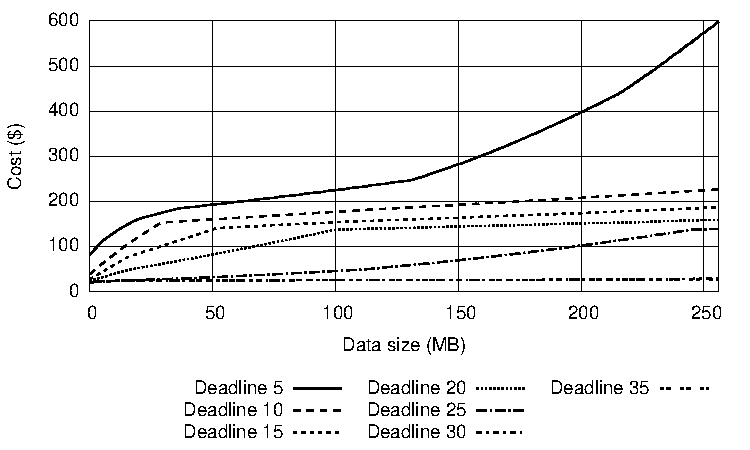
\includegraphics[width=\columnwidth]{BagOfTasks/cost_vs_data_size}
     \caption{Cost as a function of data size for different
     deadlines.\label{fig:bot:cost_vs_data_size}}
  \end{figure} 
  
  Fig.~\ref{fig:bot:cost_vs_data_size} presents these results from a perspective
  where each curve shows how the cost depends on data size for varying
  deadlines.
  
  \begin{figure}[tb]
     \centering 
     \begin{subfigure}[b]{0.49\textwidth}
       \centering       
       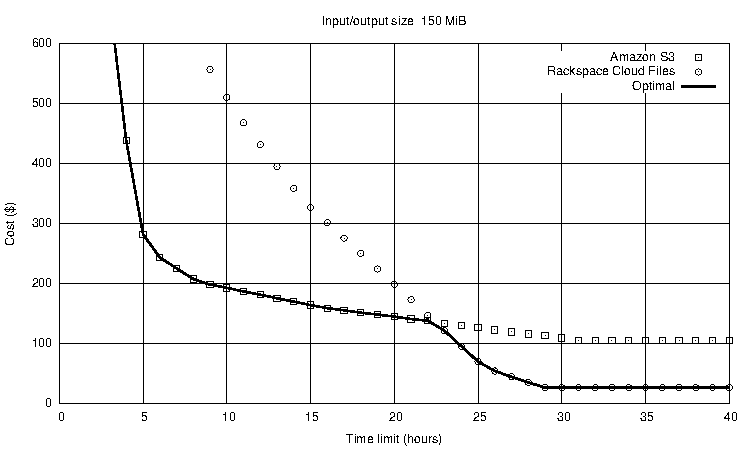
\includegraphics[width=\textwidth]{BagOfTasks/deadline-cost-150}
       \caption{Cost as a function of deadline}
     \end{subfigure}     
     \begin{subfigure}[b]{0.49\textwidth}
       \centering       
       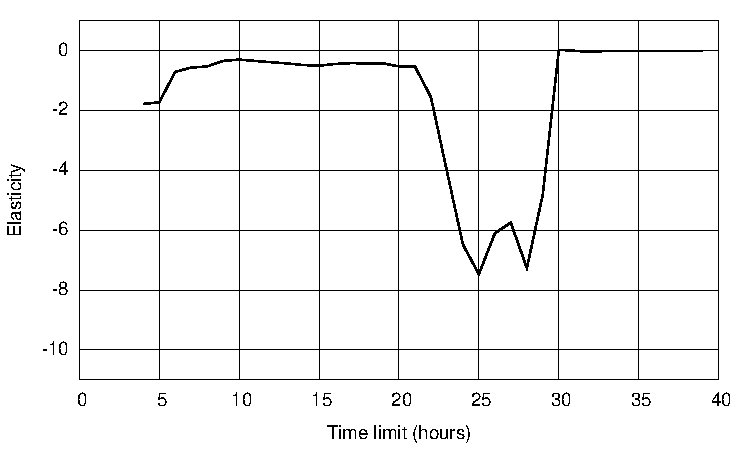
\includegraphics[width=\textwidth]{BagOfTasks/deadline-elasticity-150}
       \caption{Elasticity of cost versus deadline}
     \end{subfigure}     
     \caption{Sensitivity of costs in response to changes in deadline}
     \label{fig:bot:elasticity}
  \end{figure} 
  % 
  One of the questions that our model can help answer is how the changes in
  cost are sensitive to the changes of deadline. Fig.~\ref{fig:bot:elasticity} shows
  the cost function as well as corresponding elasticity, which is computed as:
  $E f(x) = \frac{x}{f(x)} f'(x)$, where in this case $f$ is cost and $x$ is
  deadline. Elasticity gives the information on what is the percentage change
  of cost in response to the percentage change of deadline. The function has
  negative values, since the cost decreases with the increase of deadline. It
  is interesting to see in which ranges the elasticity has larger absolute
  value, which corresponds to more steep cost function. Here we can see that
  the elasticity grows for short deadlines and close to the deadline of 25
  hours, which is the point where the solution cannot use only the VM instances
  from most cost-effective clouds and requires more expensive ones to meet the
  deadline.
  
  Identifying such ranges with high absolute value of elasticity is important
  for potential users of the cloud system, including researchers (end users) or
  resellers (brokers). The end user can for example observe that changing the
  deadline from 40 to 30 hours or even from 20 to 10 hours will not incur much
  additional cost. However, changing the deadline from 30 to 20 hours is very
  costly, so it should be avoided. On the other hand, the situation looks
  different from the perspective of a reseller, who buys cloud resources from
  providers and offers them to end-users in order to make profit. The reseller
  can for example offer to compute the given set of tasks in 20 hours for \$150
  with minimal profit, but it can also offer to complete the same set of tasks
  in 30 hours for \$50. Such price can seem attractive to the end user who pays
  1/3 of the price for increasing the deadline by 50\%, but it is in fact very
  beneficial for the reseller, whose profit reaches 100\%. Such cost analysis
  is an important aspect of planning large computing experiments on cloud
  infrastructures.

\section{Impact of dynamic environment}
\label{sec:bot:dynamic}
    
  As stated in section~\ref{sec:bot:appmodel}, we assume that execution time,
  transfer rate and data access time for all the tasks are constant. However,
  in real environments the actual runtime of tasks will vary. The goal of the
  following simulation experiment was to estimate the impact of this runtime
  variation on the quality of results obtained using our optimization model.
  
  For all the task assignment solutions presented in Fig.~\ref{fig:bot:sensitivity-surface} 
  we add runtime variations to the task runtimes in the following way. For each task
  we generate a random error in the range from $-v$ to $v$ using uniform distribution,
  where $v$ is the runtime variation range. We tested values of $v=10\%, 20\%, 30\%, 40\%, 50\%$. 
  Such modified task runtimes are then used to calculate the actual runtime and cost of 
  VM. Due to variation of task runtimes, it is possible that some computations may not 
  finish before the deadline (time overrun) and that the cost of additional VM-hours
  may need to be paid (cost overrun).

  We assume that task size variations include also
  variations of data transfer time. We don't take into account variations of
  data transfer costs, since the transfer costs for each task depend linearly
  on data size, so the aggregated impact of positive and negative variations
  cancels to nearly $0$.
  
  \begin{figure}[tb]
     \centering
     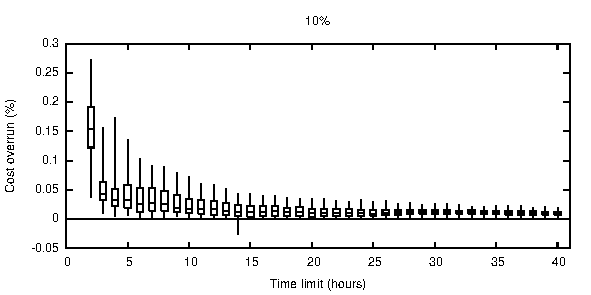
\includegraphics[width=\columnwidth]{BagOfTasks/tolerance-extended-10-2-cost-relative}  
     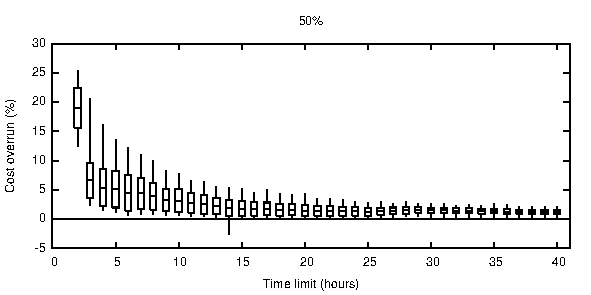
\includegraphics[width=\columnwidth]{BagOfTasks/tolerance-extended-50-2-cost-relative}  
 	   \caption{Impact of runtime variation on cost overrun as a function of deadline. 
 	   Results obtained for random variation of task runtime in the range from $-10\%$ to $+10\%$ (top)
 	   and from $-50\%$ to $+50\%$ (bottom). }
 	   \label{fig:bot:dynamic-cost}
  \end{figure} 
  
  Fig.~\ref{fig:bot:dynamic-cost} shows the cost overrun with 10\% and 50\%  of runtime
  variation range.  The boxplots for each deadline represent averaged
  results for the data sizes from 0 to 256 MiB as in
  Fig.~\ref{fig:bot:sensitivity-surface}, with box boundaries at quartiles
  and whiskers at maximum and minimum values. We observe that the highest
  overruns are for the shortest deadlines, which results from the fact that
  when each VM instance runs only for a few hours, then the additional hour
  will incur relatively high additional cost. On the other hand, for longer
  deadlines the cost of additional VM-hour becomes less significant. We also
  observe that the aggregated impact of positive and negative variations in
  task execution time may cancel to nearly $0$ and in some cases the cost
  overrun may be negative.

  \begin{figure}[tb]
     \centering
     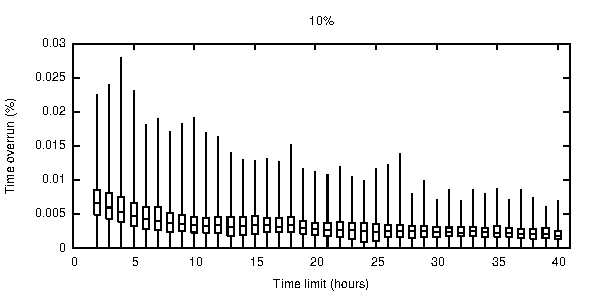
\includegraphics[width=\columnwidth]{BagOfTasks/tolerance-extended-10-2-overrun-relative}  
     
   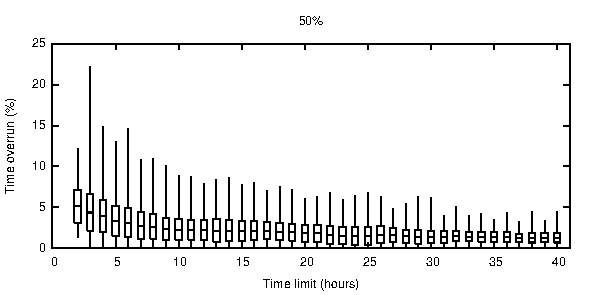
\includegraphics[width=\columnwidth]{BagOfTasks/tolerance-extended-50-2-overrun-relative}  
 	   \caption{Impact of runtime variation on deadline overrun as a function of deadline. 
 	   Results obtained for random variation of task runtime in the range from $ -10\%$ to $10\%$ (top)
 	   and from $-50\%$ to $+50\%$ (bottom). }
 	   \label{fig:bot:dynamic-time}
  \end{figure} 

  In a similar way Fig.~\ref{fig:bot:dynamic-time} shows the deadline overrun in
  the presence of runtime variations. We can observe that the deadline overrun
  is much smaller than cost overrun. This means that the actual finish time of
  all tasks is not significantly affected by the runtime variation, due to the
  cancellation effect. We observe that even for high variations in the range
  from $-50\%$ to $50\%$ the actual runtime rarely exceeds the deadline by
  more than 10\%. This overrun can be thus easily compensated by solving the
  optimization problem with a respectively shorter deadline giving a safety
  margin in the case of expected high variations of actual task runtimes. Similar estimation is also possible in the case when the application consists of many tasks of similar size which distribution in known in advance. 
	


\section{Summary}

\todo{In this chapter…}
	
} % Command scope

{ % Command scope


\newcommand{\INSTANCE}{I}
\newcommand{\STORAGE}{S}
\newcommand{\PROVIDER}{P}
\newcommand{\PROVIDERINSTANCES}{PI}
\newcommand{\LOCALSTORAGE}{LS}

\newcommand{\LAYER}{L}
\newcommand{\TASK}{G}


\newcommand{\instancePrice}{p^I}
\newcommand{\ccu}{ccu}
\newcommand{\instanceTransferPriceIn}{p^{Iin}}
\newcommand{\instanceTransferPriceOut}{p^{Iout}}
\newcommand{\storageTransferPriceOut}{p^{Sout}}
\newcommand{\storageTransferPriceIn}{p^{Sin}}
\newcommand{\transferRate}{r}


\newcommand{\taskCount}{A^{tot}}
\newcommand{\transferTime}{t^{net}}
\newcommand{\execTime}{t^x}
\newcommand{\dataSizeIn}{d^{in}}
\newcommand{\dataSizeOut}{d^{out}}
\newcommand{\requestPrice}{p^{R}}
\newcommand{\workflowDeadline}{t^D}
\newcommand{\instanceDeadline}{t^d}
\newcommand{\unitTime}{t^u}
\newcommand{\transferCost}{c^T}
\newcommand{\tasksPerDeadline}{a^d}
\newcommand{\timeQuantum}{t^q}
\newcommand{\tasksPerTimeQuantum}{a^q}
\newcommand{\providerMaxMachines}{n^{Pmax}}
\newcommand{\instanceMaxMachines}{n^{Imax}}

\newcommand{\NumberInstances}{N}
\newcommand{\TaskAssignment}{A}
\newcommand{\DataAssignment}{D}
\newcommand{\TailTaskHours}{R}
\newcommand{\HasTail}{H}

\newcommand{\instanceSet}{I^{idx}}
\newcommand{\InstanceTasks}{T}
\newcommand{\InstanceHours}{H}
\newcommand{\InstanceActive}{A}
\newcommand{\LayerDeadline}{D}
\newcommand{\LayerTime}{D^t}

\chapter{Workflow optimization}
\label{chap:formulation-workflows} 
\lhead{Chapter \ref{chap:formulation-workflows}. \emph{Workflow optimization}}

    In this chapter we discuss optimization of scientific applications that may be represented as workflows. In Section \ref{sec:workflow:appmodel} we discuss the details of scietific workflows. Then in Section \ref{sec:workflow:problem} we formulate optimization problem using AMPL by defining the data, variables, constraints and the objective. Finally, in we evaluate in Section \ref{sec:workflow:evaluation} by scheduling example workflows from Workflow Generator Gallery.
  
    \section{Application model}
    \label{sec:workflow:appmodel}
    
    As described in Section \ref{intro:workflow}, a scientific workflow describes the dependencies between tasks and in most cases may be represented as directed acyclic graph (DAG), where nodes represent tasks and edges represent task dependencies. 
    
    There are different approaches to optimize workflow scheduling (see Chapter \ref{chap:state-of-art}). Mathematical programming allows to describe the model mathematically and use a set of available optimization solvers. On the other hand, an attempt to apply this method to the general problem of scheduling large-scale workflows on heterogeneous cloud resources would be impractical due to the problem complexity, therefore simplified models need to be analyzed. Optimization models can be simplified in several ways. We may simplify application model, infrastructure model or make certain assumptions on output schedule.
    
    In this model we assume that workflow is represented as a DAG. We also assume that a workflow is divided into several levels (layers) that can be executed sequentially and tasks within one level do not depend on each other (see Fig.~\ref{fig:workflow:appmodel}). Each layer represents a bag of tasks that can be partitioned in several groups (e.g. application A, application B, etc.) that share computational cost and input/output size. We assume that only one task group is executed on a specific cloud instance (VM). This forbids instance sharing between multiple layers, which means that each application needs its own specific VM template with a preconfigured environment.

    \begin{figure}[tb]
        \centering 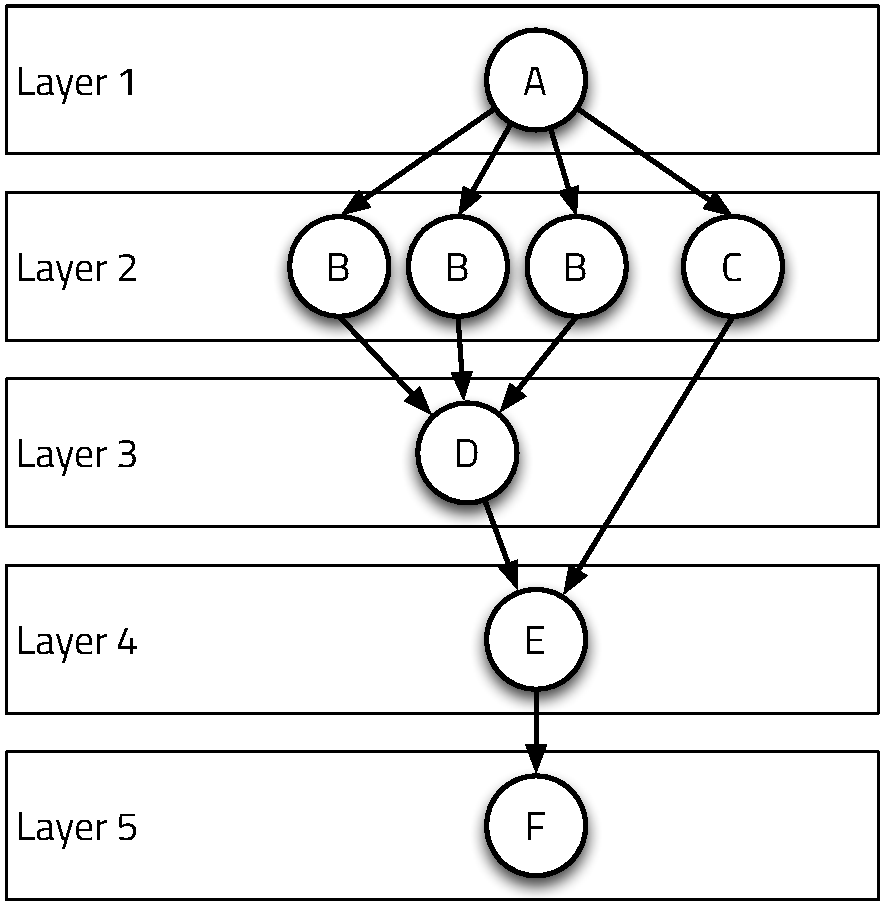
\includegraphics[width=0.5\columnwidth]{Workflow/workflow}
        \caption{Example application structure}
        \label{fig:workflow:appmodel}
    \end{figure}
    
    In this model we will use the same infrastructure model as presented in Section~\ref{sec:bot:cloudmodel}.
  
    \section{Problem formulation using AMPL}
    \label{sec:workflow:problem}
  
    To perform optimization of the total cost, Mixed Integer Problem (MIP) is formulated and implemented in A Mathematical Programming Language (AMPL)~\cite{Fourer2002}.  AMPL requires us to specify input data sets and variables to define the search space, as well as constraints and objective function to be optimized.
    
    \subsection{Input data}
    \label{sec:workflow:problem:input}
     
    The formulation requires the following input sets, which represent the infrastructure model, in a similar way as we approached the problem in Chapter~\ref{chap:bot}:
    \begin{itemize}
        \item $\STORAGE = \{s3, cloudfiles\}$ -- defines available cloud storage
        sites,
        \item $\PROVIDER = \{amazon, rackspace, \dotsc\}$ -- defines
        possible computing cloud providers,
        \item $\INSTANCE = \{m1.small, \dots, gg.1gb, \dotsc\}$ -- defines
        instance types,
        \item $\PROVIDERINSTANCES_{p} \subset \INSTANCE$ -- instances that
        belong to provider $\PROVIDER_p$,
        \item $\LOCALSTORAGE_{s} \subset \PROVIDER$ -- compute cloud providers
        that are local to storage platform $\STORAGE_s$.
    \end{itemize}        
        
    Each instance type $\INSTANCE_i$ is described by the following parameters:
    \begin{itemize}
        \item $\instancePrice_i$ -- fee in \$ for running instance $\INSTANCE_i$
        for one hour,
        \item $\ccu_i$ -- performance of instance in CloudHarmony Compute Units
        (CCU),
        \item $\instanceTransferPriceOut_i$ and $\instanceTransferPriceIn_i$ --
        price for non-local data transfer to and from the instance, in \$ per
        MiB (1 MiB = $1024*1024$ Bytes)
    \end{itemize}
    
    Storage sites are characterized by:
    \begin{itemize}
        \item $\storageTransferPriceOut_s$ and $\storageTransferPriceIn_s$
        characterize price in \$ per MiB for non local data transfer.
    \end{itemize}
    
    Additionally we need to provide data transfer rates in MiB per second between
    storage and instances by defining function $\transferRate_{i,s} > 0$ .
    
  
    Our application model is different from the one in~Chapter~\ref{chap:bot} because it groups tasks into layers:

    \begin{itemize}
        \item $\LAYER$  -- set of layers,
        \item $\TASK$   -- set of tasks groups,
        \item $\TASK_l$ -- set of tasks groups belonging to layer $l$, 
        \item $\taskCount_t$ -- number of tasks in group $t$,
        \item $\execTime_t$ -- execution time in hours of a single task of group $t$ on 1 CCU
        machine,
        \item $\dataSizeIn_t$ and $\dataSizeOut_t$ -- data size for input and
        output of one task $t$ in MiB,
        \item $\requestPrice$ -- price per request for queuing service, such as Amazon SQS, required to execute a single task,
        \item $\workflowDeadline$ -- total time for completing workflow (deadline).
    \end{itemize} 
    
    \subsection{Auxiliary parameters}
    \label{sec:workflow:problem:auxiliary}
    
    A set of precomputed parameters which are derived from the main input parameters of the model includes:
     \begin{align}
         \transferTime_{i,s} &= \frac{\dataSizeIn+\dataSizeOut}{\transferRate_{i,s} \cdot 3600}  \\
         \label{workflow:unitTime}\unitTime_{i,s} &= \frac{\execTime}{\ccu_i} + \transferTime_{i,s}  \\
         \begin{split}
             \transferCost_{i,s} &= (\dataSizeOut \cdot
             (\instanceTransferPriceOut_i + \storageTransferPriceIn_s) \\ & +
             \dataSizeIn \cdot (\storageTransferPriceOut_s+\instanceTransferPriceIn_i)) \end{split} \\
     \end{align}
    \begin{itemize}
        \item $\transferTime_{i,s}$ -- {\em transfer time}: time for data transfer between
        $\INSTANCE_i$ and $\STORAGE_s$,
        \item $\unitTime_{i,s}$ -- {\em unit time}: time for processing a task
        on instance $\INSTANCE_i$ using storage $\STORAGE_s$ that includes computing and
        data transfer time (in hours),
        \item $\transferCost_{i,s}$ -- cost of data transfer between instance
        $\INSTANCE_i$ and storage $\STORAGE_s$,
        \item $\instanceSet_i$ -- set of possible instance $\INSTANCE_i$ indexes (from $0$ to $\instanceMaxMachines_i - 1$).
    \end{itemize}
   
    \subsection{Variables}
    \label{sec:workflow:problem:variables}
    Variables that will be optimized and define the solution space are:
    \begin{itemize}
        \item $\InstanceActive_{t,i,x}$ -- binary, $1$ iif (if and only if) instance $\INSTANCE_i$ with index $x$ is launched to process task group $\TASK_t$, otherwise $0$;
        \item $\InstanceHours_{t,i,x}$ -- integer, for how many hours is instance launched;
        \item $\InstanceTasks_{t,i,x}$ -- integer, how many tasks of $\TASK_t$ are processed on that instance,
        \item $\LayerTime_l$ -- actual computation time for $\LAYER_l$,
        \item $\LayerDeadline_l$ -- integer, maximal number of hours that instances are allowed to run in $\LAYER_l$.
    \end{itemize}
    
    \subsection{Formulation of objectives}
    \label{sec:workflow:problem:objective}
    
    Cost of running one task including instance and transfer cost is:

    \begin{align}
        \left(\transferTime + \unitTime\right) \cdot \instancePrice + 
        \dataSizeIn \cdot \left(\storageTransferPriceOut + \instanceTransferPriceIn\right) + 
        \dataSizeOut \cdot \left(\instanceTransferPriceOut + \storageTransferPriceIn\right) + 
        \requestPrice
    \end{align}

    while the objective function represents the total cost of running multiple
    tasks of the application on the cloud infrastructure is defined as:
    
    \begin{align}    
    \begin{split}
        \underset{\text{total cost}}{\text{minimize}} \sum \limits_{t \in \TASK, i \in \INSTANCE, x \in \instanceSet_i}  ( & 
                    (\instancePrice_i * \InstanceHours_{t,i,x} + \requestPrice + \transferCost_{i,s})*\InstanceTasks_{t,i,x} 
                   )
    \end{split}
    \end{align}
      
   subject to the constraints:
   \nopagebreak 
   \begin{align}
       \label{workflow:cLayerDeadline} \mathop\sum\limits_{l \in \LAYER} & \LayerDeadline_l \leq \workflowDeadline
       \\
       \label{workflow:cLayerTime}     \mathop\forall\limits_{l \in \LAYER} & \LayerTime_l \leq \LayerDeadline_l \leq \LayerTime_l + 1
       \\
       \label{workflow:cInstancesActiveHours} \mathop\forall\limits_{t \in \TASK, i \in \INSTANCE, x \in \instanceSet_i} & 
         \InstanceActive_{t,i,x} \leq \InstanceHours_{t,i,x} \leq  \InstanceActive_{t,i,x} \cdot \workflowDeadline
       \\
       \label{workflow:cInstancesActiveTasks} \mathop\forall\limits_{t \in \TASK, i \in \INSTANCE, x \in \instanceSet_i} &
         \InstanceActive_{t,i,x} \leq \InstanceTasks_{t,i,x} \InstanceActive_{t,i,x} \cdot \taskCount_t
       \\
       \label{workflow:cEnsureLayerDeadline} \mathop\forall\limits_{t \in \TASK, i \in \INSTANCE, x \in \instanceSet_i} &
         \InstanceHours_{t,i,x} \leq \LayerDeadline_l
       \\ 
       \label{workflow:cEnsureLayerTime} \mathop\forall\limits_{l \in \LAYER, t \in \TASK_l, i \in \INSTANCE, x \in \instanceSet_i} &
         \InstanceTasks_{t,i,x} \cdot \unitTime_{t,i,s} \leq \LayerTime_l
       \\       
       \label{workflow:cEnoughProcessingPower} \mathop\forall\limits_{t \in \TASK, i \in \INSTANCE, x \in \instanceSet_i} &
         \InstanceTasks_{t,i,x} \cdot \unitTime_{t,i,s} \leq \InstanceHours_{t,i,x} \InstanceTasks_{t,i,x} \cdot \unitTime_{t,i,s} + 1\\
       \\         
       \label{workflow:cProcessAllTasks} \mathop\forall\limits_{t \in \TASK} &
         \mathop\sum\limits_{i \in \INSTANCE, x \in \instanceSet_i} \InstanceTasks_{t,i,x} = \taskCount_t
       \\
       \label{workflow:cSymmetricSolutions1} \mathop\forall\limits_{t \in \TASK, i \in \INSTANCE, x \in \left\{1 .. \left(\instanceMaxMachines_i - 1\right)\right\}} & 
         \InstanceHours_{t,i,x} \leq \InstanceHours_{t,i,x-1} \\        
       \label{workflow:cSymmetricSolutions2} \mathop\forall\limits_{t \in \TASK, i \in \INSTANCE, x \in \left\{1 .. \left(\instanceMaxMachines_i - 1\right)\right\}} & 
         \InstanceActive_{t,i,x} \leq \InstanceActive_{t,i,x-1}\\ 
       \label{workflow:cSymmetricSolutions3} \mathop\forall\limits_{t \in \TASK, i \in \INSTANCE, x \in \left\{1 .. \left(\instanceMaxMachines_i - 1\right)\right\}} &
         \InstanceTasks_{t,i,x} \leq \InstanceTasks_{t,i,x-1}
       \\
       \label{workflow:cProviderLimits} \mathop\forall\limits_{l \in \LAYER, p \in \PROVIDER} &
         \mathop\sum\limits_{i \in \PROVIDERINSTANCES_p, t \in \TASK_l, x \in \instanceSet_i} \InstanceActive_{t,i,x} \leq \providerMaxMachines_p
    \end{align}
    
    Interpretation of the constraints is the following:
    \begin{itemize}
        \item(\ref{workflow:cLayerDeadline}) ensures that workflow finishes in given deadline,
        \item(\ref{workflow:cLayerTime}) fix that $\LayerDeadline = \ceil{\LayerTime}$,
        \item(\ref{workflow:cInstancesActiveHours}) ensure that $\InstanceHours$ may be allocated only iif $\InstanceActive$ is $1$,
        \item(\ref{workflow:cInstancesActiveTasks}) ensure that $\InstanceTasks$ may be allocated only iif $\InstanceActive$ is $1$,
        \item(\ref{workflow:cEnsureLayerDeadline}) enforces layer deadline on instances runtime,
        \item(\ref{workflow:cEnsureLayerTime}) enforces layer finishes work in $\LayerTime$,
        \item(\ref{workflow:cEnoughProcessingPower}) adjust $\InstanceHours$ respectively to $\InstanceTasks$ in order to make sure that all the instances run for enough time to process all tasks allocated to them we require,
        \item(\ref{workflow:cProcessAllTasks}) ensures that all tasks are processed,
        \item(\ref{workflow:cSymmetricSolutions1} to \ref{workflow:cSymmetricSolutions3}) reject symmetric solutions,
        \item(\ref{workflow:cProviderLimits}) enforces instance limits per cloud.
    \end{itemize}
    
    To keep this model in MIP class I had to take different approach than in previous model, and schedule each virtual machine instance separately. The drawback of this approach is that we need to increase the number of decision variables. The search space is also divided by storage provider. Additionally, the deadline becomes a variable with upper bound as it may happen that shorter deadline may actually give a cheaper solution (see Fig.~\ref{fig:workflow:genome-500-ratio} and its discussion).
    
    
    \section{Evaluation}
    \label{sec:workflow:evaluation}

    To evaluate our model on realistic data, we use CloudHarmony~\cite{CloudHarmony} benchmarks to parameterize the infrastructure model, and we use the Workflow  Generator Gallery workflows~\cite{Bharathi08} as test applications.

    In the infrastructure model we assumed that we have 4 public cloud providers (Amazon EC2, RackSpace, GoGrid and ElasticHosts) and a private cloud with 0 cost. The infrastructure has two object storage services, S3 that is local to EC2 and CloudFiles that is local to RackSpace, so data transfers between local compute and storage are free. 

    We tested our model with all application types from the gallery: Montage, CyberShake, Epigenomics, LIGO and SIPHT for all available workflow sizes (from 50 to 1000 tasks per workflows, up to 5000 tasks in the case of SIPHT workflow). We varied the deadline from 1 to 30 hours with 1-hour increment. We solve the problem for two cases, depending on whether the data is stored on Amazon S3 or on RackSpace CloudFiles.
  
    \begin{figure}[b] 
       \centering
       \begin{subfigure}[b]{0.49\textwidth}  
         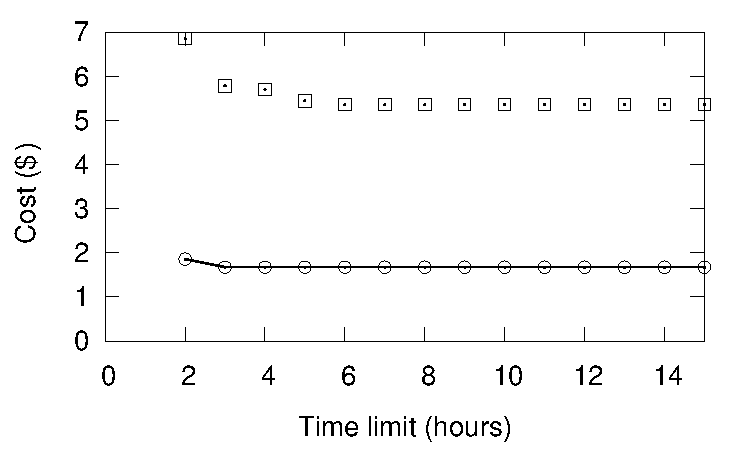
\includegraphics[width=\textwidth]{Workflow/Genome400-deadline_cost}
         \caption{400 tasks, 1 GiB data size}
         \label{fig:workflow:genome-400}
       \end{subfigure}
       \begin{subfigure}[b]{0.49\textwidth}
         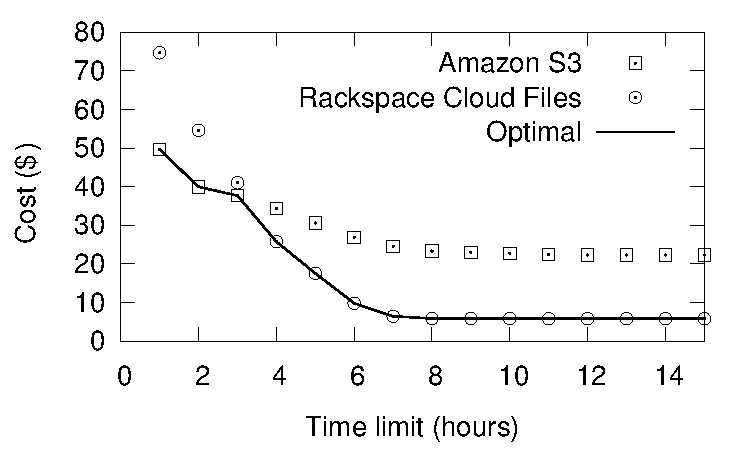
\includegraphics[width=\textwidth]{Workflow/Genome500-deadline_cost}
         \caption{500 tasks, 4 GiB data size}
         \label{fig:workflow:genome-500}
       \end{subfigure}
       \caption{\label{fig:workflow:genome}Result of the optimization procedure for the Epigenomics application.}
    \end{figure}  

    Fig.~\ref{fig:workflow:genome} shows the example results obtained for the Epigenomics application and workflows of two sizes (400 and 500 tasks). For longer deadlines the private cloud instances and the cheapest RackSpace instances are used so the cost is low when using CloudFiles. For shorter deadlines the cost grows rapidly, since we reach the limit of 15 instances per cloud and additional instances must be spawned on a different provider, making the transfer costs higher. This effect is amplified in Fig.~\ref{fig:workflow:genome-500}, which differs from Fig.~\ref{fig:workflow:genome-400} not only by the number of tasks but also by the data size of one layer. This means that the transfer costs are growing more rapidly, so it becomes more economical to store the data on Amazon EC2 that provides more powerful instances required for short deadlines.
    
    \begin{figure}[tb]
       \centering 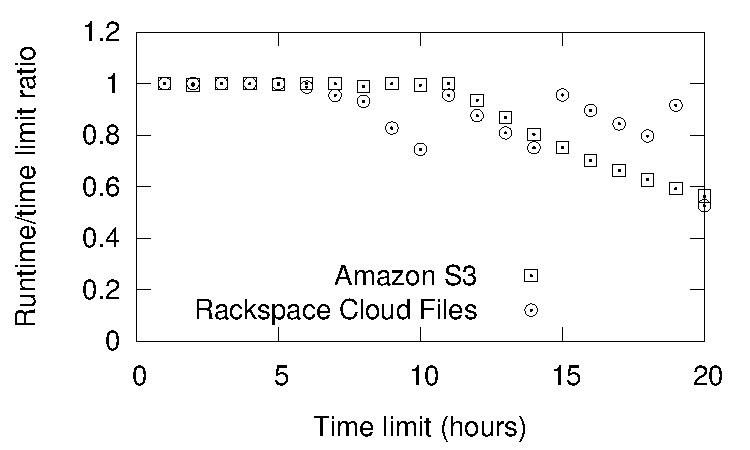
\includegraphics[width=0.7\textwidth]{Workflow/Genome500-time_ratio}
       \caption{Ratio of actual completion time to deadline for Epigenomics workflow with 500 tasks.
       \label{fig:workflow:genome-500-ratio}}
    \end{figure}
    
    One interesting feature of our model is that for longer deadlines it can find the cost-optimal solutions that have shorter workflow completion time than the requested deadline. This effect can be observed in Fig.~\ref{fig:workflow:genome-500-ratio} and is caused by the fact that for long deadlines the simple solution is to run the application on a set of the least expensive machines. 
    
    \begin{figure}[tb] 
       \centering       
       \begin{subfigure}[b]{0.49\textwidth}  
         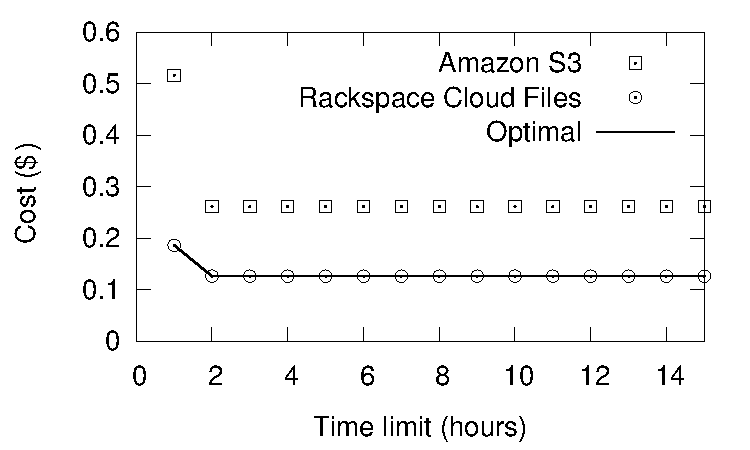
\includegraphics[width=\linewidth]{Workflow/CYBERSHAKE-500-deadline_cost}
         \caption{CyberShake, 500 tasks}
         \label{fig:workflow:cybershake-500}
       \end{subfigure}
      \begin{subfigure}[b]{0.49\textwidth}  
        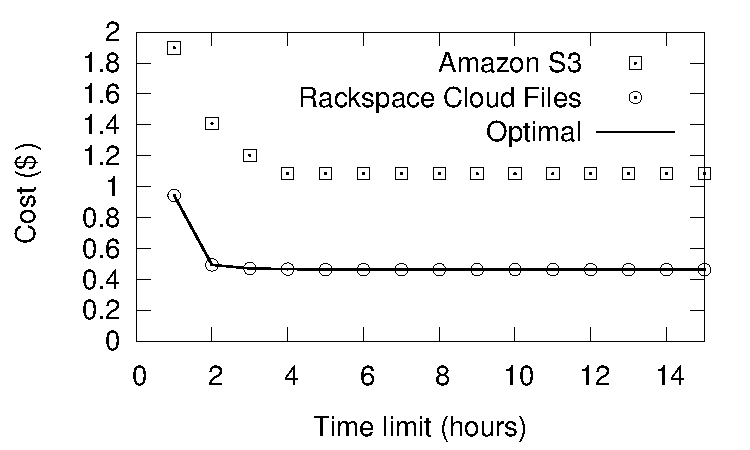
\includegraphics[width=\linewidth]{Workflow/LIGO-500-deadline_cost}
        \caption{LIGO, 500 tasks}
        \label{fig:workflow:ligo-500}
      \end{subfigure} \\ 
      \begin{subfigure}[b]{0.49\textwidth}  
        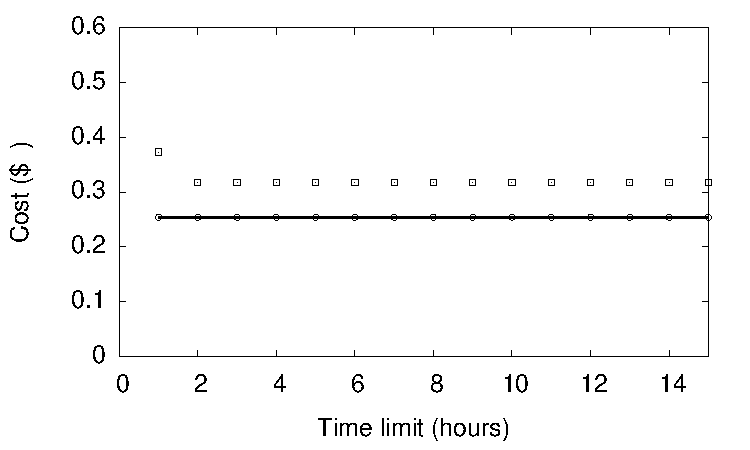
\includegraphics[width=\linewidth]{Workflow/MONTAGE-500-deadline_cost}
        \caption{Montage, 500 tasks}
        \label{fig:workflow:montage-500}
      \end{subfigure}             
      \begin{subfigure}[b]{0.49\textwidth}  
        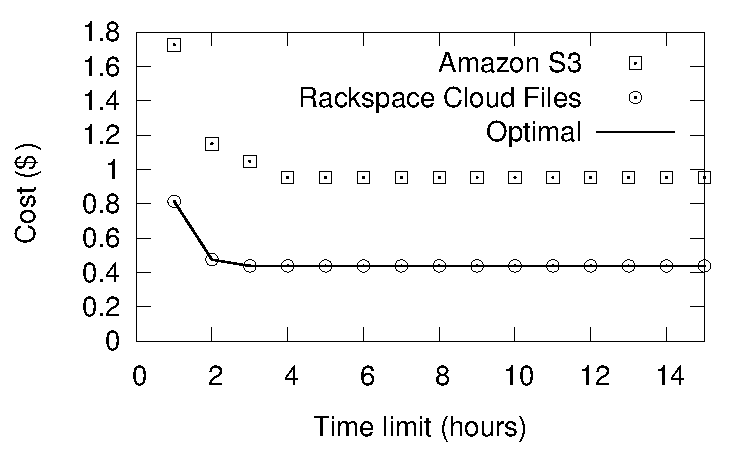
\includegraphics[width=\linewidth]{Workflow/SIPHT-500-deadline_cost}
        \caption{SIPHT, 500 tasks}
        \label{fig:workflow:sipht-500}
      \end{subfigure}\\
      \begin{subfigure}[b]{0.49\textwidth}  
        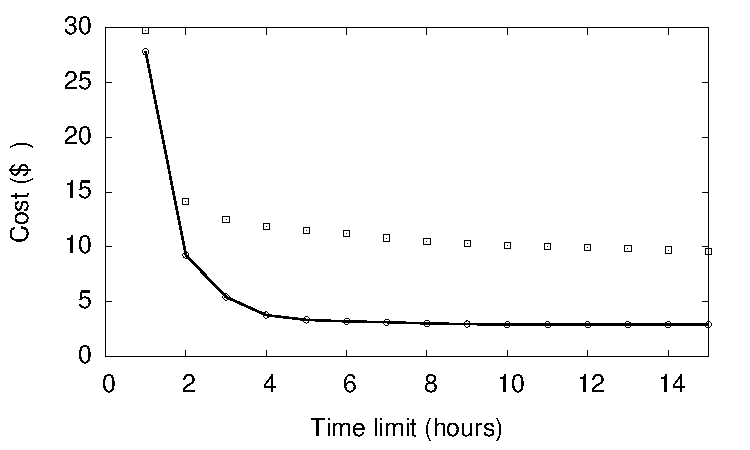
\includegraphics[width=\linewidth]{Workflow/SIPHT-5000-deadline_cost}
        \caption{SIPHT, 5000 tasks}
        \label{fig:workflow:sipht-5000}
      \end{subfigure}
      \caption{\label{fig:other}Optimal cost found by the model for different application.}
    \end{figure}  
    \todo{add more pics that did not fit into PPAM}
    Figures \ref{fig:workflow:cybershake-500} to \ref{fig:workflow:sipht-5000}  show results obtained for other workflows. These workflows are relatively small and even for short deadlines our model is able to schedule tasks to be executed in a very short time on cheapest instances on a single cloud, this results in flat characteristics.
    
    To investigate how the model behaves for workflows with the same structure, but with much longer run times of tasks, we run the optimization for Montage workflow with tasks $1000 \times$ longer. This corresponds to the scenario where tasks are in the order of hours instead of seconds. The sample results in Fig.~\ref{fig:workflow:montage-500x1000} show how the cost increases much steeply with shorter deadlines, illustrating the trade-off between time and cost. The difference between Figs.~\ref{fig:workflow:montage-500}~and~\ref{fig:workflow:montage-500x1000} illustrates that the model is more useful for workflows when tasks are of granularity that is similar to the granularity of the (hourly) billing cycle of cloud providers.    

    \begin{figure}[tb]
       \centering 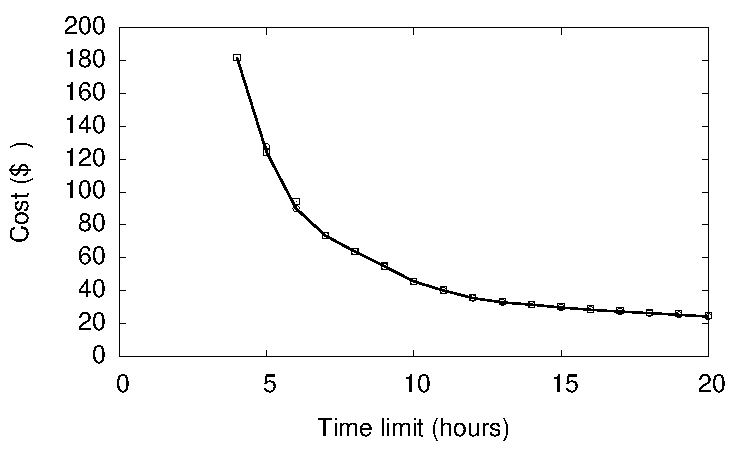
\includegraphics[width=0.7\textwidth]{Workflow/MONTAGE-500x1000-deadline_cost}
       \caption{Optimal cost obtained by the model for Montage 500 workflow with tasks runtimes artificailly 
       multiplied by 1000.
       \label{fig:workflow:montage-500x1000}}
    \end{figure}

    \begin{figure}[tb] 
       \centering
       
       \begin{subfigure}[b]{0.49\textwidth}  
         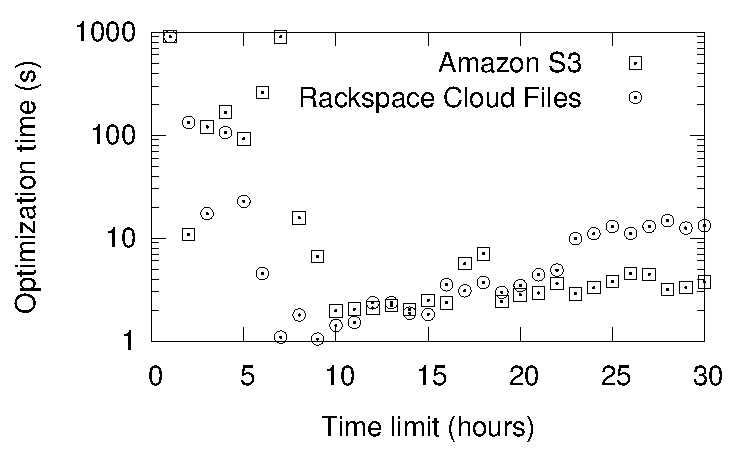
\includegraphics[width=\linewidth]{Workflow/Genome600-wall_time}
         \caption{Epigenomics, 600 tasks}
         \label{fig:workflow:genome-600-opttime}
       \end{subfigure}
       \begin{subfigure}[b]{0.49\textwidth}
         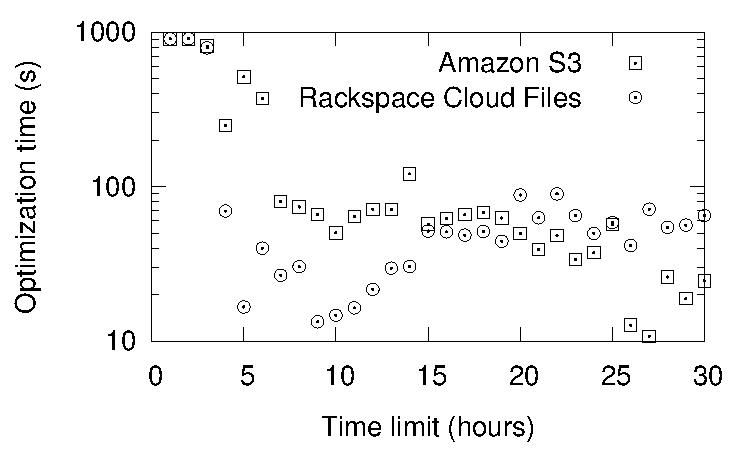
\includegraphics[width=\linewidth]{Workflow/SIPHT-5000-wall_time}
         \caption{SIPHT, 5000 tasks}
         \label{fig:workflow:sipht-5000-opttime}
       \end{subfigure}
       
       \caption{Solver execution wall time.}
    \end{figure}
  
    
    The run time of the optimization algorithm for workflows with up to 1000 tasks ranges from few seconds up to 4 minutes using the CPLEX~\cite{cplex} solver running on a server with 4 16-core 2.3 GHz AMD Opteron processors (model 6276), with a limit set to 32 cores. Fig.~\ref{fig:workflow:genome-600-opttime} shows that the time becomes much higher for shorter deadlines and increases for very long deadlines. This is correlated with size of search space: the longer the deadline, the search space is larger, while for shorter deadlines the problem has a very small set of acceptable solutions.  The problem becomes more severe for bigger and more complex workflows like SIPHT as optimization time becomes very high (Fig.~\ref{fig:workflow:sipht-5000-opttime}).
    
} % Command scope
\chapter{Conclusions and future work}
\label{chap:conclusions} 
\lhead{Chapter \ref{chap:conclusions}. \emph{Conclusions and future work}}

\section{Conclusions}

The results presented in this thesis illustrate typical problems when making decisions on deployment planning on clouds and how they can be addressed using optimization techniques. The major goal of this thesis was the theoretical and practical investigation of optimization of resource allocation on the cloud by using integer linear programming tools and methods. The theoretical part of the goal was accomplished by exploration on the cloud computing, existing workflow scheduling, resource allocation algorithms and mathematical programming that was presented in first three chapters. 

To practically evaluate integer linear programming approach to the problem, we defined application model of bag of tasks applications and workflows. We also defined the infrastructure model of multiple heterogenous clouds, including private and public ones. The optimization model takes into account the cost of compute instances and data transfer that proved to have significant contribution to the total. The mixed integer nonlinear optimization models were then implemented in AMPL modeling language and optimized with Cbc and CPLEX solvers. The models were evaluated in terms of results, performance and solution stability by performing a parameter sweep and analyzing the results. 

The integer linear programming proved to be approach for resource allocation for the scientific computing. The AMPL appeared to be friendly tool to perform such optimization.

\section{Future work}

As a future work we could perform experiments on real cloud infrastructure by using real applications and data sets. That would allow us to better understand cloud infrastructure deployment issues and see how dynamic environment affects offline resource allocation.

Furthermore, the infrastructure model should be extended to better reflect cloud infrastructure caveats and new cloud features such as the 5-minute billing cycle introduced by Cloud-Sigma. Additional cloud services should be also considered, as they may be also used by scientific applications

Additionally, the mathematical programming approach could be applied as a subproblem solving method for heuristic algorithm. For that, we should investigate multi-stage optimization algorithms.

Last, but not least, the workflow model performance is subject to be improved by either simplifying application or infrastructure model or by applying other modeling techniques.




%----------------------------------------------------------------------------------------
%	THESIS CONTENT - APPENDICES
%----------------------------------------------------------------------------------------

\addtocontents{toc}{\vspace{2em}} % Add a gap in the Contents, for aesthetics

\appendix % Cue to tell LaTeX that the following 'chapters' are Appendices

% Include the appendices of the thesis as separate files from the Appendices folder
% Uncomment the lines as you write the Appendices

% % Appendix A

\chapter{Appendix Title Here} % Main appendix title

\label{AppendixA} % For referencing this appendix elsewhere, use \ref{AppendixA}

\lhead{Appendix A. \emph{Appendix Title Here}} % This is for the header on each page - perhaps a shortened title

Write your Appendix content here.
%\input{./Appendices/AppendixB}
%\input{./Appendices/AppendixC}

\addtocontents{toc}{\vspace{2em}} % Add a gap in the Contents, for aesthetics

\backmatter

%----------------------------------------------------------------------------------------
%	BIBLIOGRAPHY
%----------------------------------------------------------------------------------------

\label{Bibliography}

\lhead{\emph{Bibliography}} % Change the page header to say "Bibliography"

\bibliographystyle{unsrtnat} % Use the "unsrtnat" BibTeX style for formatting the Bibliography

\bibliography{Bibliography} % The references (bibliography) information are stored in the file named "Bibliography.bib"

\end{document}  